%!TEX TS-program = xelatex

\documentclass[t]{beamer}  % [t], [c], или [b] --- вертикальное выравнивание на слайдах (верх, центр, низ)
%\documentclass[t, handout]{beamer} % Раздаточный материал (на слайдах всё сразу)
%\documentclass[aspectratio=169, t]{beamer} % Соотношение сторон

\usepackage{epstopdf}

%\usetheme{Berkeley} % Тема оформления
%\usetheme{Bergen}
%\usetheme{Szeged}

%\usecolortheme{beaver} % Цветовая схема
%\useinnertheme{circles}
%\useinnertheme{rectangles}

\usepackage{HSE-theme/beamerthemeHSE} % Подгружаем тему


%%% Работа с русским языком
\usepackage{cmap}					% поиск в PDF
\usepackage{mathtext} 				% русские буквы в формулах
\usepackage[T2A]{fontenc}			% кодировка
\usepackage[utf8]{inputenc}			% кодировка исходного текста
%%% Работа с русским языком и шрифтами
\usepackage[english,russian]{babel}   % загружает пакет многоязыковой вёрстки


%%% Дополнительная работа с математикой
\usepackage{amsmath,amsfonts,amssymb,amsthm,mathtools} % AMS
\usepackage{icomma} % "Умная" запятая: $0,2$ --- число, $0, 2$ --- перечисление

%% Номера формул
%\mathtoolsset{showonlyrefs=true} % Показывать номера только у тех формул, на которые есть \eqref{} в тексте.
%\usepackage{leqno} % Нумерация формул слева

%% Свои команды
\DeclareMathOperator{\sgn}{\mathop{sgn}}

%% Перенос знаков в формулах (по Львовскому)
\newcommand*{\hm}[1]{#1\nobreak\discretionary{}
	{\hbox{$\mathsurround=0pt #1$}}{}}

%%% Работа с картинками
\usepackage{graphicx}  % Для вставки рисунков
\graphicspath{{images/}{images2/}}  % папки с картинками
\setlength\fboxsep{3pt} % Отступ рамки \fbox{} от рисунка
\setlength\fboxrule{1pt} % Толщина линий рамки \fbox{}
\usepackage{wrapfig} % Обтекание рисунков текстом
\usepackage{caption}


%%% Работа с таблицами
\usepackage{array,tabularx,tabulary,booktabs} % Дополнительная работа с таблицами
\usepackage{longtable}  % Длинные таблицы
\usepackage{multirow} % Слияние строк в таблице

%%% Программирование
\usepackage{etoolbox} % логические операторы

%%% Другие пакеты
\usepackage{lastpage} % Узнать, сколько всего страниц в документе.
\usepackage{soul} % Модификаторы начертания
\usepackage{csquotes} % Еще инструменты для ссылок
%\usepackage[style=authoryear,maxcitenames=2,backend=biber,sorting=nty]{biblatex}
\usepackage{multicol} % Несколько колонок

%%% Картинки
\usepackage{tikz} % Работа с графикой
\usepackage{pgfplots}
\usepackage{pgfplotstable}
\usepackage{verbatim}
\usetikzlibrary{fadings}
\usepackage[outline]{contour}
\usepackage{pifont} 

\usepackage{chngcntr} % нумерация графиков и таблиц по секциям
\counterwithin{table}{section}
\counterwithin{figure}{section}

\usepackage{listings}

\lstdefinelanguage{Rust}{
  sensitive=true,
  morekeywords=[1]{
    break, continue, else, for, if, loop, match, return, while,
  },
  morekeywords=[2]{
    crate, fn, async, mod, pub, use, self, Self,
    struct, enum, const, static, let, mut, ref, type, impl,
    trait, where, as, dyn, move,
  },
  morekeywords=[3]{
    bool, char, i8, i16, i32, i64, isize, u8, u16, u32, u64, usize, f32, f64, str, String,
  },
  morekeywords=[4]{
    Ok, Err, Some, None,
  },
  morekeywords=[5]{
    await,
  },
  keywordstyle=[5]{\color{purple}},
  morecomment=[s]{/*}{*/},
  morecomment=[l]//,
  morestring=[b]",
  morestring=[b]r",
  morestring=[b]'',
}

\lstset{
  language=Rust,
  basicstyle=\ttfamily,
  keywordstyle=\color{blue},
  stringstyle=\color{red},
  commentstyle=\color{green},
  showstringspaces=false,
  breaklines=true,
  frame=none,
}


\lstnewenvironment{rustcode}[1][]{
  \lstset{
    language=Rust,
    basicstyle=\ttfamily,
    keywordstyle=\color{blue},
    stringstyle=\color{red},
    commentstyle=\color{gray},
    showstringspaces=false,
    breaklines=true,
    % frame=single,
    #1
  }
}{}

\usepackage{setspace}
\usepackage{color}



\title{Реализация поддержки асинхронного программирования для фреймворка \texttt{DSLab}}
\author[Артём Макогон]{\footnotesize Выполнил: Макогон Артём Аркадьевич, БПМИ206 \\[5pt]   Руководитель: Сухорослов Олег Викторович, к.т.н, доцент НИУ ВШЭ}
\date{\today}
% \institute[Высшая школа экономики]{National Research University\\ 
	% <<Higher School of Economics>>}



\begin{document}
	
	\begin{frame}
		\maketitle
	\end{frame}
	
    \section{Введение}
    \subsection{Описание предметной области}

	\begin{frame}[fragile]
		\frametitle{\insertsection} 
		\framesubtitle{\insertsubsection}

		\begin{columns}
			\begin{column}{0.5\linewidth}
				\vspace{0.5cm}
				\begin{itemize}
					\item Большой объем данных/вычислений 
					\item Надежность
					\item Масштабируемость
				\end{itemize}
				\alt<2>{
					{ \hspace{2cm} \large $\Downarrow$ } 
					\begin{itemize}
						\item[\small\textgreater] Недетерминированные алгоритмы
						\item[\small\textgreater] Сложное тестирование
					\end{itemize}
				}{}
			\end{column}
			\begin{column}{0.6\linewidth}
				\vspace{1cm}
				
\includegraphics[width=\linewidth]{images/ds_intro}
			\end{column}
		\end{columns}
		
	\end{frame}

	\subsection{\texttt{DSLab}. Дискретно-событийное моделирование}

    \begin{frame}
    \frametitle{\insertsection} 
	\framesubtitle{\insertsubsection}

	\begin{figure}
		\centering
		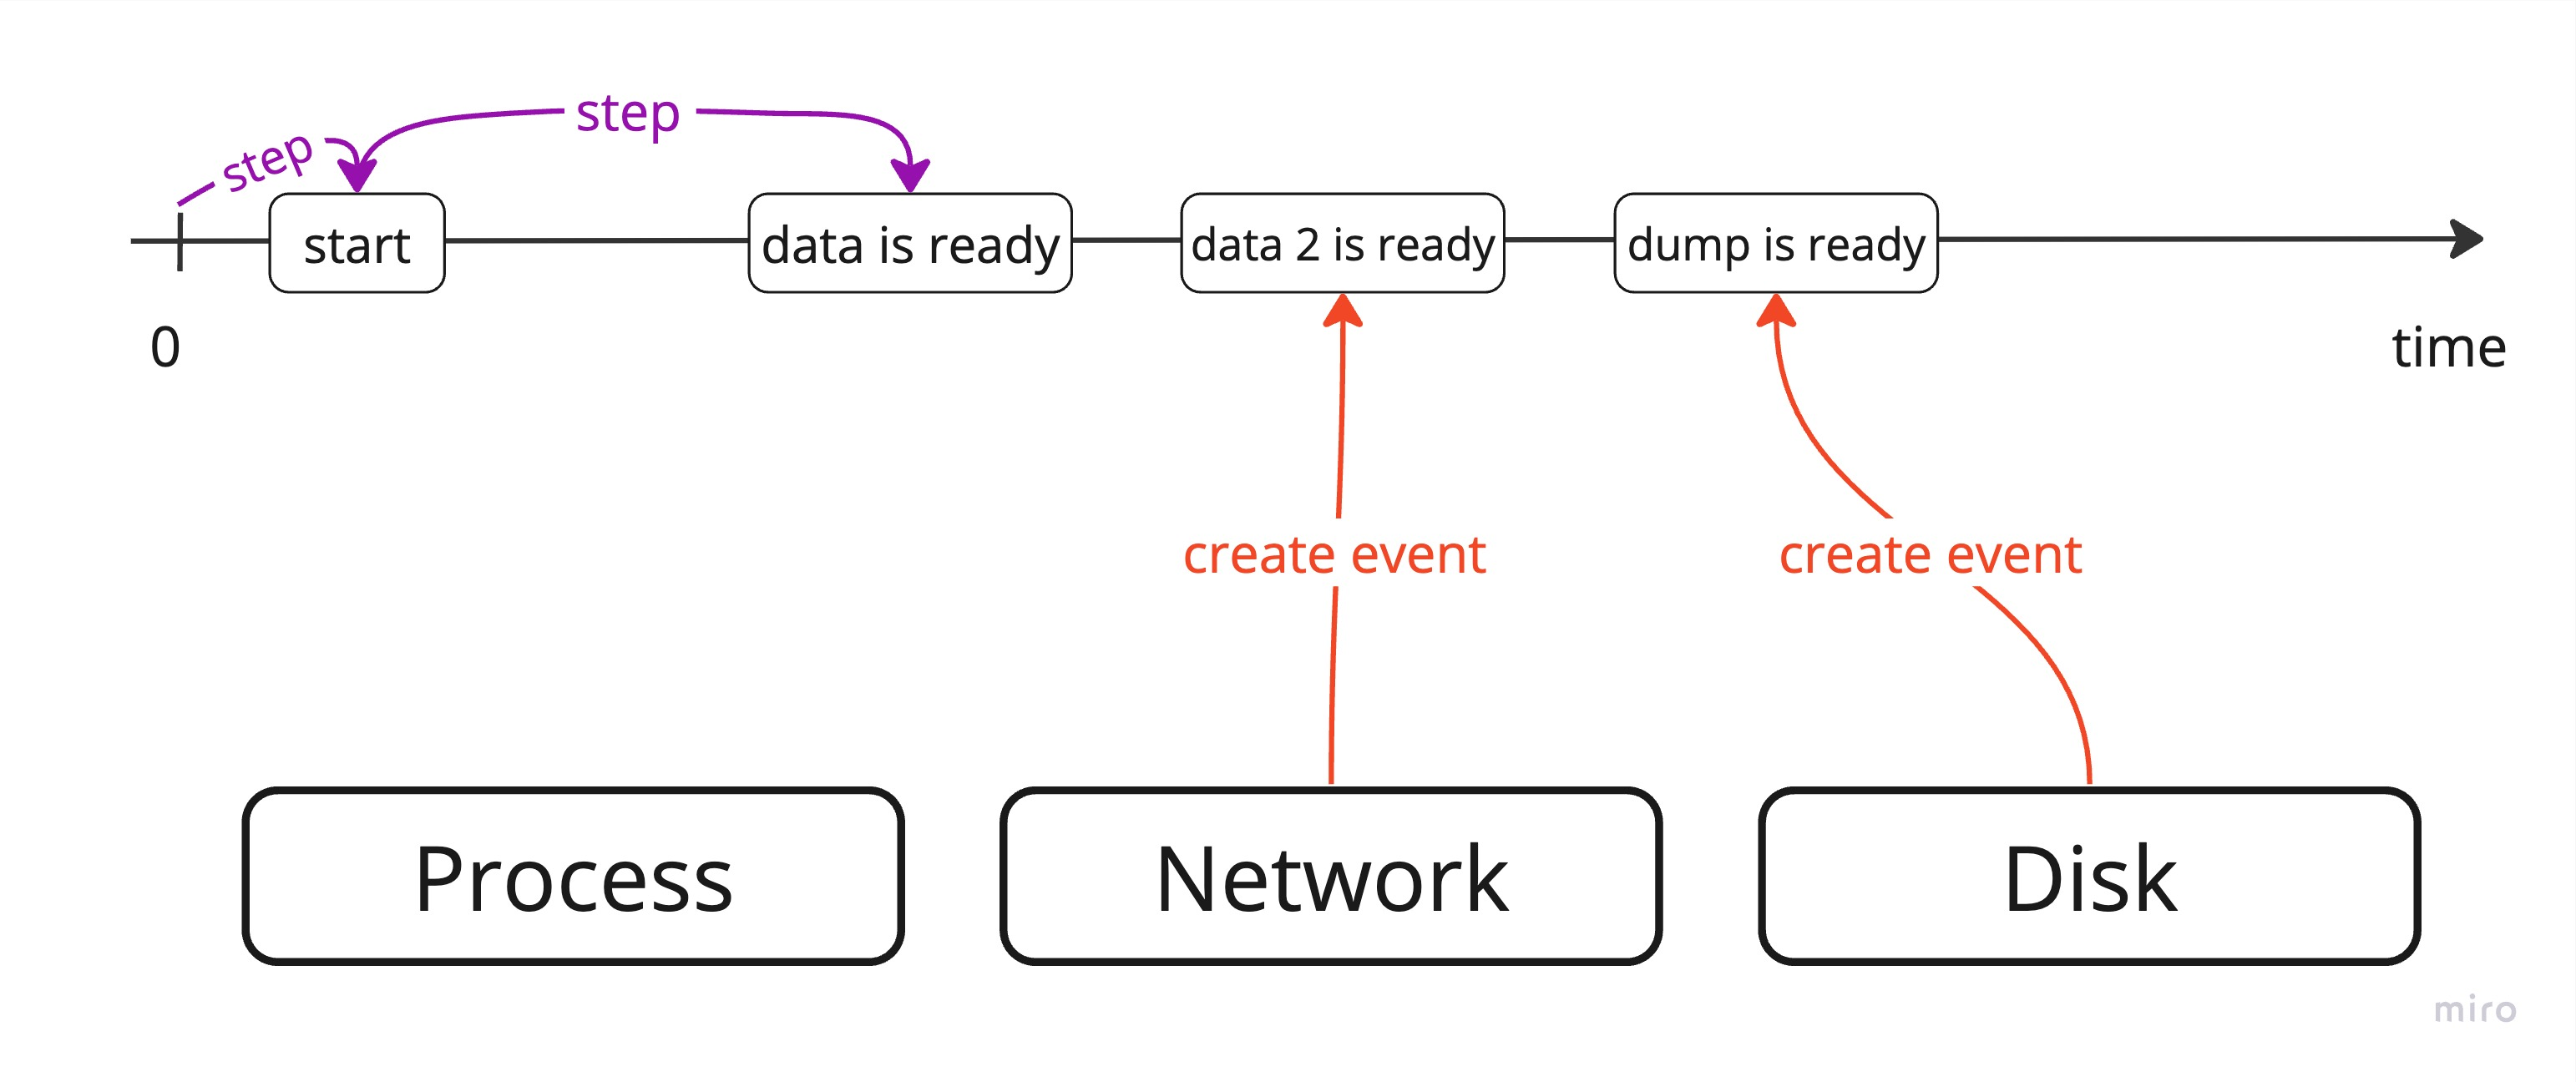
\includegraphics[width=\linewidth]{images/event_pipeline_6}
		\label{simulation}
		\caption*{Исполнение симуляции}
	\end{figure}
    \end{frame}

	\subsection{Архитектура проекта \texttt{DSLab}}
	\begin{frame}
		\frametitle{\insertsection} 
		\framesubtitle{\insertsubsection}

		\begin{figure}[H]
			\centering
			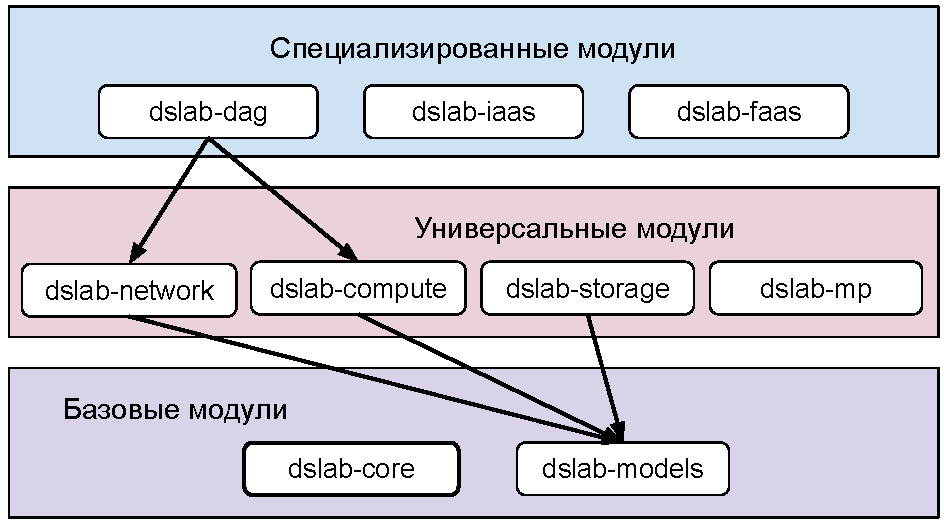
\includegraphics[width=0.9\linewidth]{images/dslab_arc}
			\caption*{Архитектура \texttt{DSLab}}
			\label{dslab_arc}
		\end{figure}
	\end{frame}


	\subsection{\texttt{Callback} модель. Фрагментированная реализация \texttt{Process}.}
	\begin{frame}[fragile]
		\frametitle{\insertsection} 
		\framesubtitle{\insertsubsection}
		\begin{columns}[c] 
			\begin{column}{0.73\textwidth} % First column
		\begin{figure}
			\scriptsize
			\centering
			\begin{rustcode}[escapeinside={(*@}{@*)}]
fn on(&mut self, event: Event) {
  cast!(match event.data {
    Start {} => {
      self.(*@\footnotesize\textcolor{OldHSEblue}{on\_start();}@*)
    }
    DownloadCompleted {data} => {
      self.(*@\footnotesize\textcolor{orange}{on\_download\_completed(data);}@*)
    }
    DiskWriteCompleted => {
      self.(*@\footnotesize\textcolor{HSEgreen}{on\_disk\_write\_completed();}@*)
    }
  })
}
			\end{rustcode}
			\caption*{Реагирование на события.}
		\end{figure}

	\end{column}
	
	\begin{column}[c]{0.24\textwidth}
		\begin{figure}
			\scriptsize
			\centering
			\begin{rustcode}[escapeinside={(*@}{@*)}]
impl Process {
  fn (*@\footnotesize\textcolor{OldHSEblue}{on...}@*) {
    (*@\tikz{\node[draw, fill=OldHSEblue, rounded corners, minimum width=1.5em, minimum height=1.5em, opacity=0.75] {};}
	@*)
  }
  fn (*@\footnotesize\textcolor{orange}{on...}@*) {
    (*@\tikz{\node[draw, fill=orange, rounded corners, minimum width=1.5em, minimum height=1.5em, opacity=0.75] {};}@*)
  }
  fn (*@\footnotesize\textcolor{HSEgreen}{on...}@*) {
    (*@\tikz{\node[draw, fill=HSEgreen, rounded corners, minimum width=1.5em, minimum height=1.5em, opacity=0.75] {};}@*)
  }
}
			\end{rustcode}
			\caption*{Реализация \texttt{callback}-ов}
		\end{figure}
	\end{column}
	\end{columns}

	\end{frame}

	\subsection{Преимущества асинхронного подхода}
	\begin{frame}[fragile]
		\frametitle{\insertsection} 
		\framesubtitle{\insertsubsection}

		\begin{figure}
			\footnotesize
			\centering
			\begin{rustcode}
async fn collect_file_from_replicas(replicas) {
  result = download_from_all(replicas).await;
	
  if result.has_quorum {
    dump_file_to_storage(result.file).await;

    send_ok_message_to_user();
  } else {
    send_reject_message_to_user();
  }
}
			\end{rustcode}
			\caption*{Псевдокод асинхронного взаимодействия компонент в симуляции}
		\end{figure}


	\end{frame}

	\subsection{Постановка задачи}
	\begin{frame}
		\frametitle{\insertsection} 
		\framesubtitle{\insertsubsection}

		\vspace{0.3cm}
		\begin{columns}
			\begin{column}{1.05\linewidth}
				\underline{Цель проекта} -- реализация поддержки асинхронного программирования для фреймворка \texttt{DSLab}. Для этого необходимо:
				\vspace{3pt}
				\begin{itemize}
					\setlength{\itemsep}{1em}
					\item Реализовать эффективное асинхронное расширение для существующего ядра \texttt{dslab-core}. Поддержать возможности:
					\begin{itemize}
						\item запустить асинхронную задачу;
						\item \texttt{<\textless}заснуть\texttt{>\textgreater} на определенное время внутри симуляции;
						\item асинхронно ждать событий от других компонент;
						\item комбинировать ожидания с помощью методов \texttt{futures}.
					\end{itemize}
					\item Добавить примеры, написать документацию и тесты.
				\end{itemize}
			\end{column}
		\end{columns}
	\end{frame}

\subsection{Дизайн и структура ядра \texttt{dslab-core}}

	\begin{frame}[fragile]
		\frametitle{\insertsection} 
		\framesubtitle{\insertsubsection}
		\vspace{-10pt}

		\begin{figure}
			\centering
			{
			\includegraphics<1>[width=\linewidth]{images/dslab_overview_1}			\includegraphics<2>[width=\linewidth]{images/dslab_overview_2}
			\includegraphics<3>[width=\linewidth]{images/dslab_overview_3}
			\includegraphics<4>[width=\linewidth]{images/dslab_overview_4}
			\includegraphics<5>[width=\linewidth]{images/dslab_overview_5}
			\includegraphics<6>[width=\linewidth]{images/dslab_overview_6}
			}
			\caption*{Внутреннее устройство \texttt{dslab-core}}
		\end{figure}
	\end{frame}



 \section{Новое \texttt{API} для пользователей}
 \subsection{Расширение \texttt{SimulationContext}}

 \begin{frame}[fragile]
	\frametitle{\insertsection} 
	\framesubtitle{\insertsubsection}

	\begin{columns}
\begin{column}[t]{1.1\linewidth}
	\vspace{-0.5cm}
	\begin{itemize}
		\setlength{\itemsep}{0.7em} 
		\item Запустить асинхронную задачу: 
		\begin{itemize}
			\item[\footnotesize\ding{58}]  \lstinline[language=Rust, basicstyle=\footnotesize\ttfamily]{fn spawn(&self, future: impl Future<Output = ()>)}
		\end{itemize}
		\item \texttt{<\textless}Заснуть\texttt{>\textgreater} на определенное время:
			\begin{itemize}
				\setlength{\itemsep}{0.5em} 
				\item[\footnotesize\ding{58}]  \lstinline[language=Rust, basicstyle=\footnotesize\ttfamily]{async fn async_wait_for(&self, timeout: f64)}
			\end{itemize}
		\item Дождаться события с \texttt{<\textless}данными\texttt{>\textgreater} типа \texttt{T} от компонента \texttt{src}:
			\begin{itemize}
				\setlength{\itemsep}{0.5em} 
				\item[\footnotesize\ding{58}] \lstinline[language=Rust,basicstyle=\footnotesize\ttfamily]{async fn async_handle_event<T>(src: Id) -> (Event, T)}
				\item[\footnotesize\ding{58}] \lstinline[language=Rust,basicstyle=\footnotesize\ttfamily]{async fn async_wait_for_event<T>(src: Id, timeout: f64) -> AwaitResult<T>}
			\end{itemize}
		\item Дождаться события с \texttt{<\textless}данными\texttt{>\textgreater} \texttt{T}, деталями \texttt{details} от \texttt{src}:
		\begin{itemize}
			\setlength{\itemsep}{0.5em} 
			\item[\footnotesize\ding{58}]\lstinline[language=Rust,basicstyle=\footnotesize\ttfamily]{async fn async_detailed_handle_event<T>(src: Id, details: u64) -> (Event, T)}
			\item[\footnotesize\ding{58}]  \lstinline[language=Rust,basicstyle=\footnotesize\ttfamily]{async fn async_detailed_wait_for_event<T>(src: Id, details: u64, timeout: f64) -> AwaitResult<T>}
		\end{itemize}
	\end{itemize}
\end{column}
\end{columns}
 \end{frame}

 \subsection{Детализированное ожидание. Пример}

 \begin{frame}[fragile]
	\frametitle{\insertsection} 
	\framesubtitle{\insertsubsection}

	\begin{columns}
		\begin{column}{1.1\linewidth}
			\begin{figure}[H]
				\footnotesize
			\begin{rustcode}
async fn process_data_transfer_request(
	&self, request: Request) {
  let request_id = self.network.send(request);
  
  self.ctx.
   async_detailed_handle_event::<DataTransferCompleted>(
    self.network.id, 
    request_id,
  ).await;
}
			\end{rustcode}
			\caption*{Использование детализированного асинхронного ожидания}
			\end{figure}
		\end{column}
	\end{columns}

 \end{frame}

 \section{Внутреннее устройство и реализация}
 \subsection{\texttt{Callback}-based модель}
 \begin{frame}[fragile]
	\frametitle{\insertsection} 
	\framesubtitle{\insertsubsection}
	\vspace{-15pt}
	\begin{figure}
		\centering
		\alt<1>{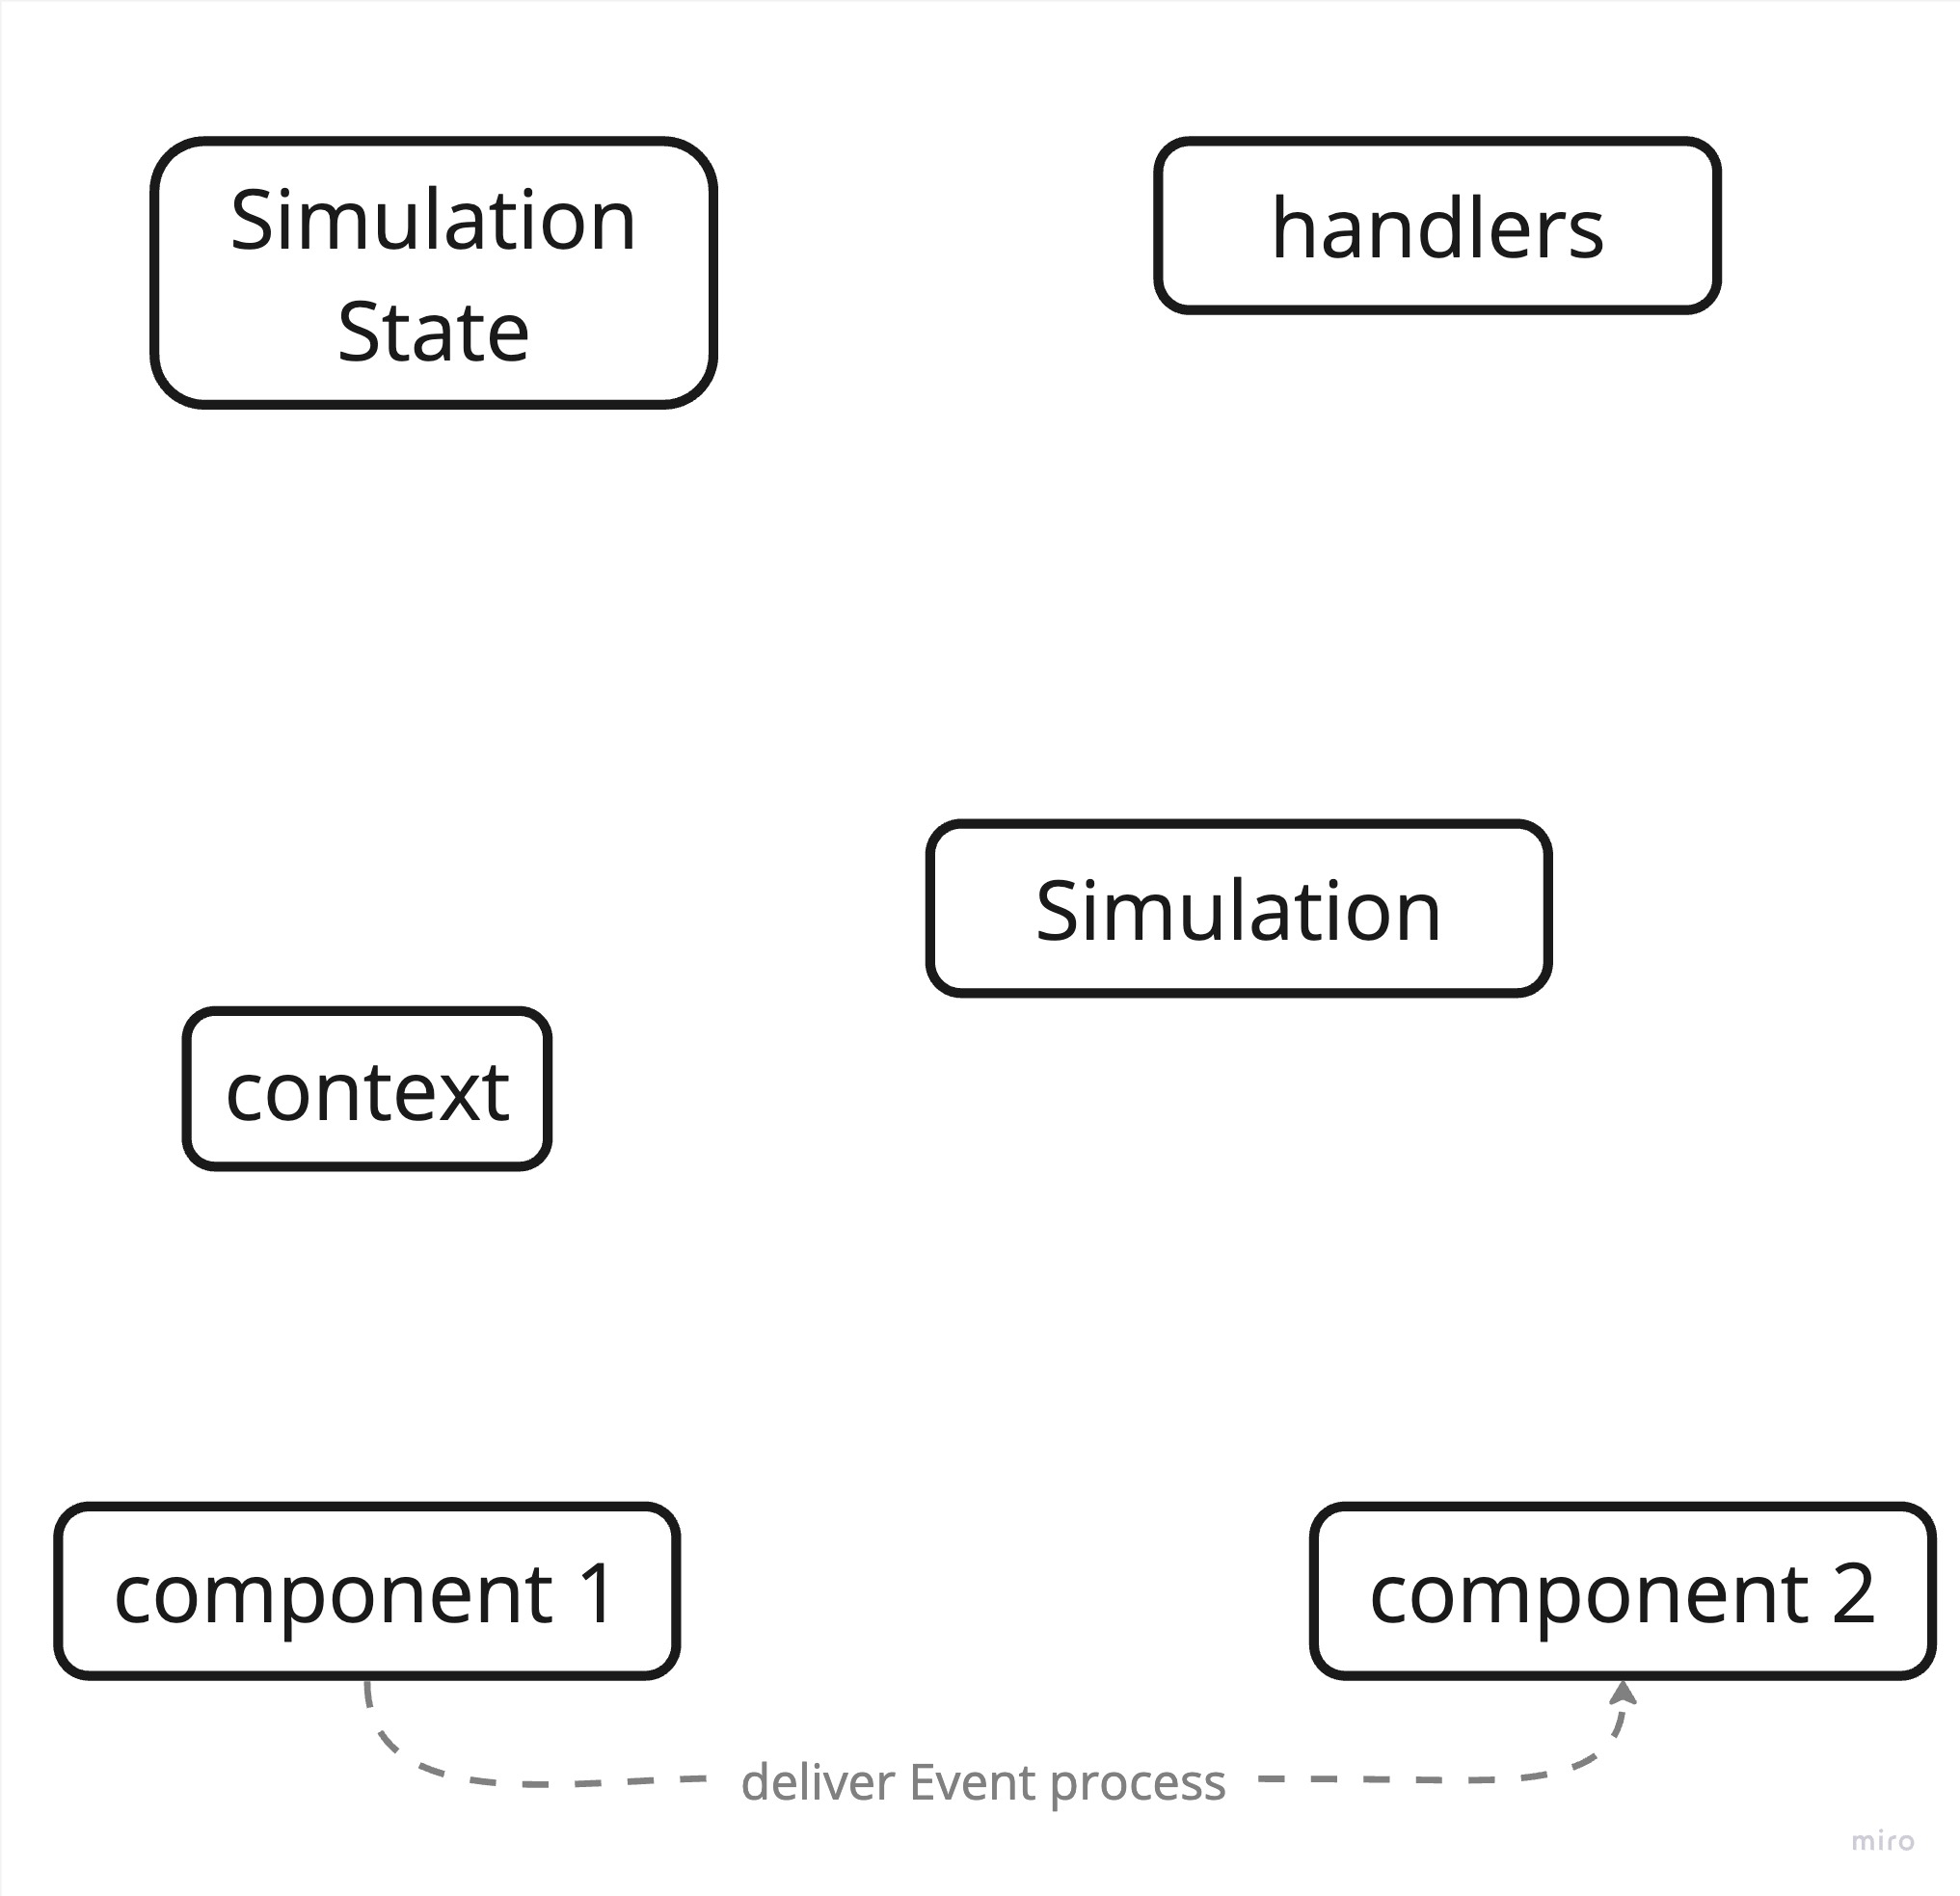
\includegraphics[width=0.72\linewidth]{images/callback_process_1}}{}
		\alt<2>{\hspace{-3.5pt}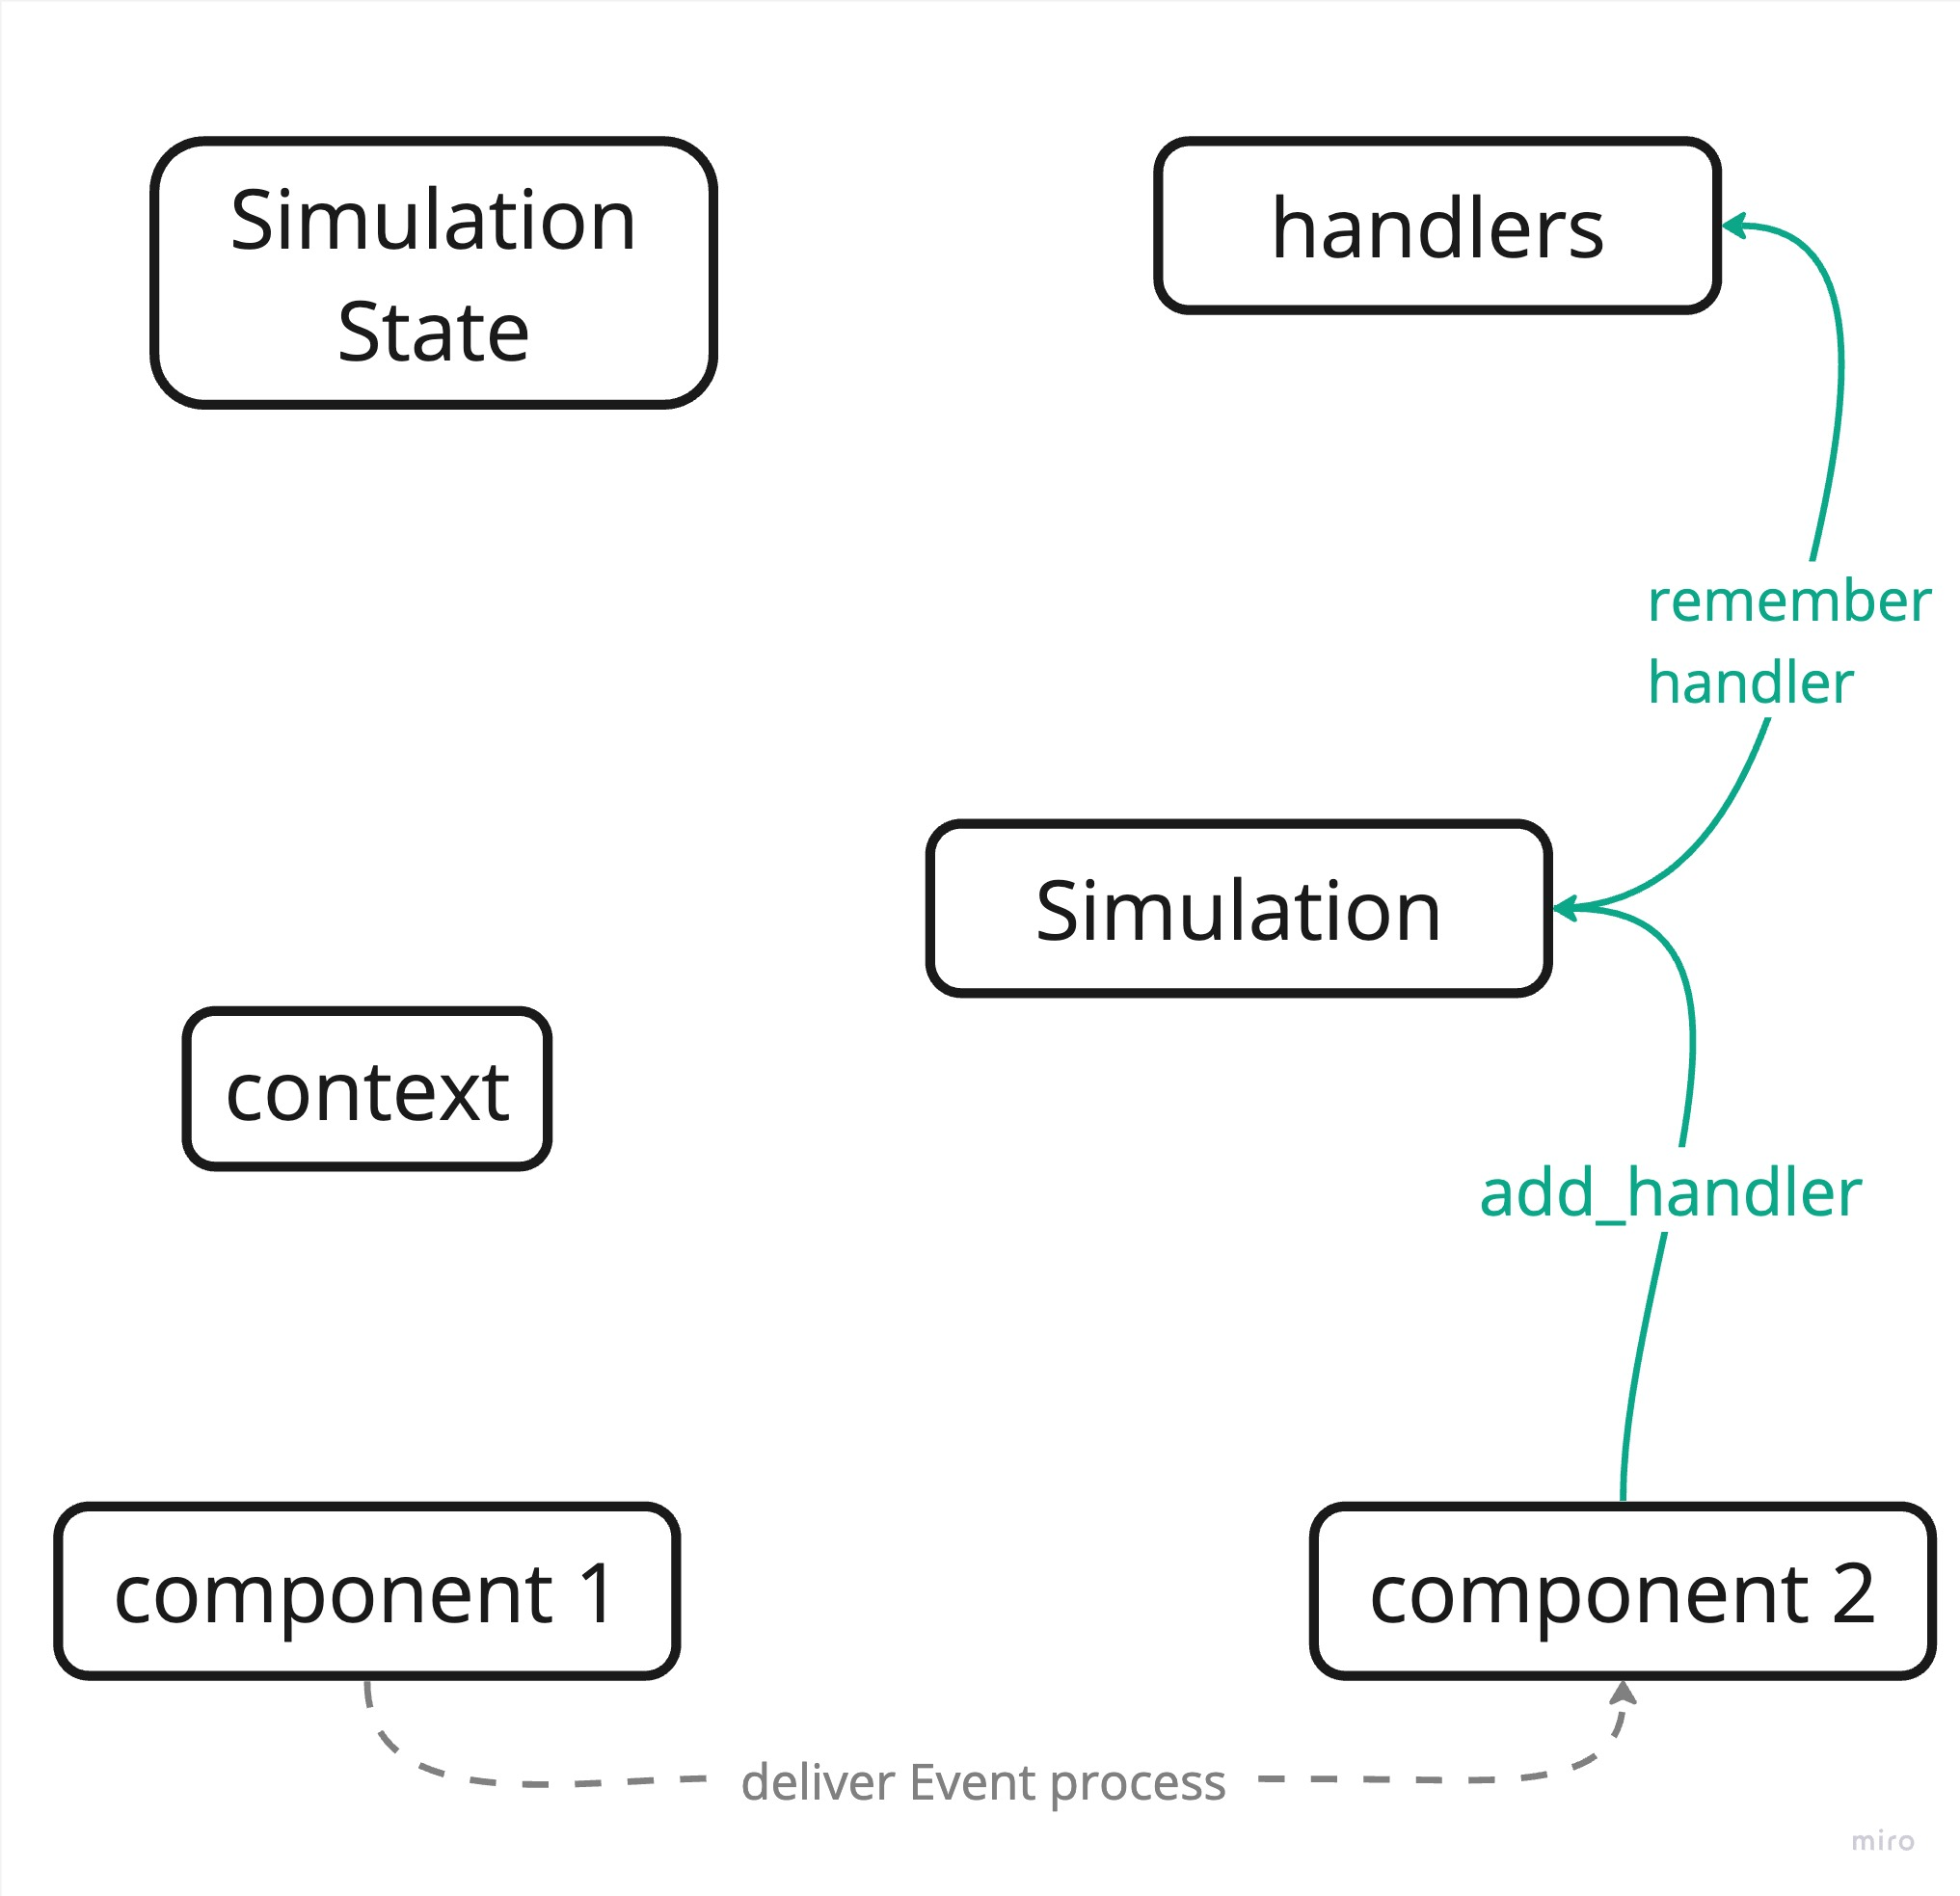
\includegraphics[width=0.72\linewidth]{images/callback_process_2}}{}
		\alt<3>{\hspace{-7pt}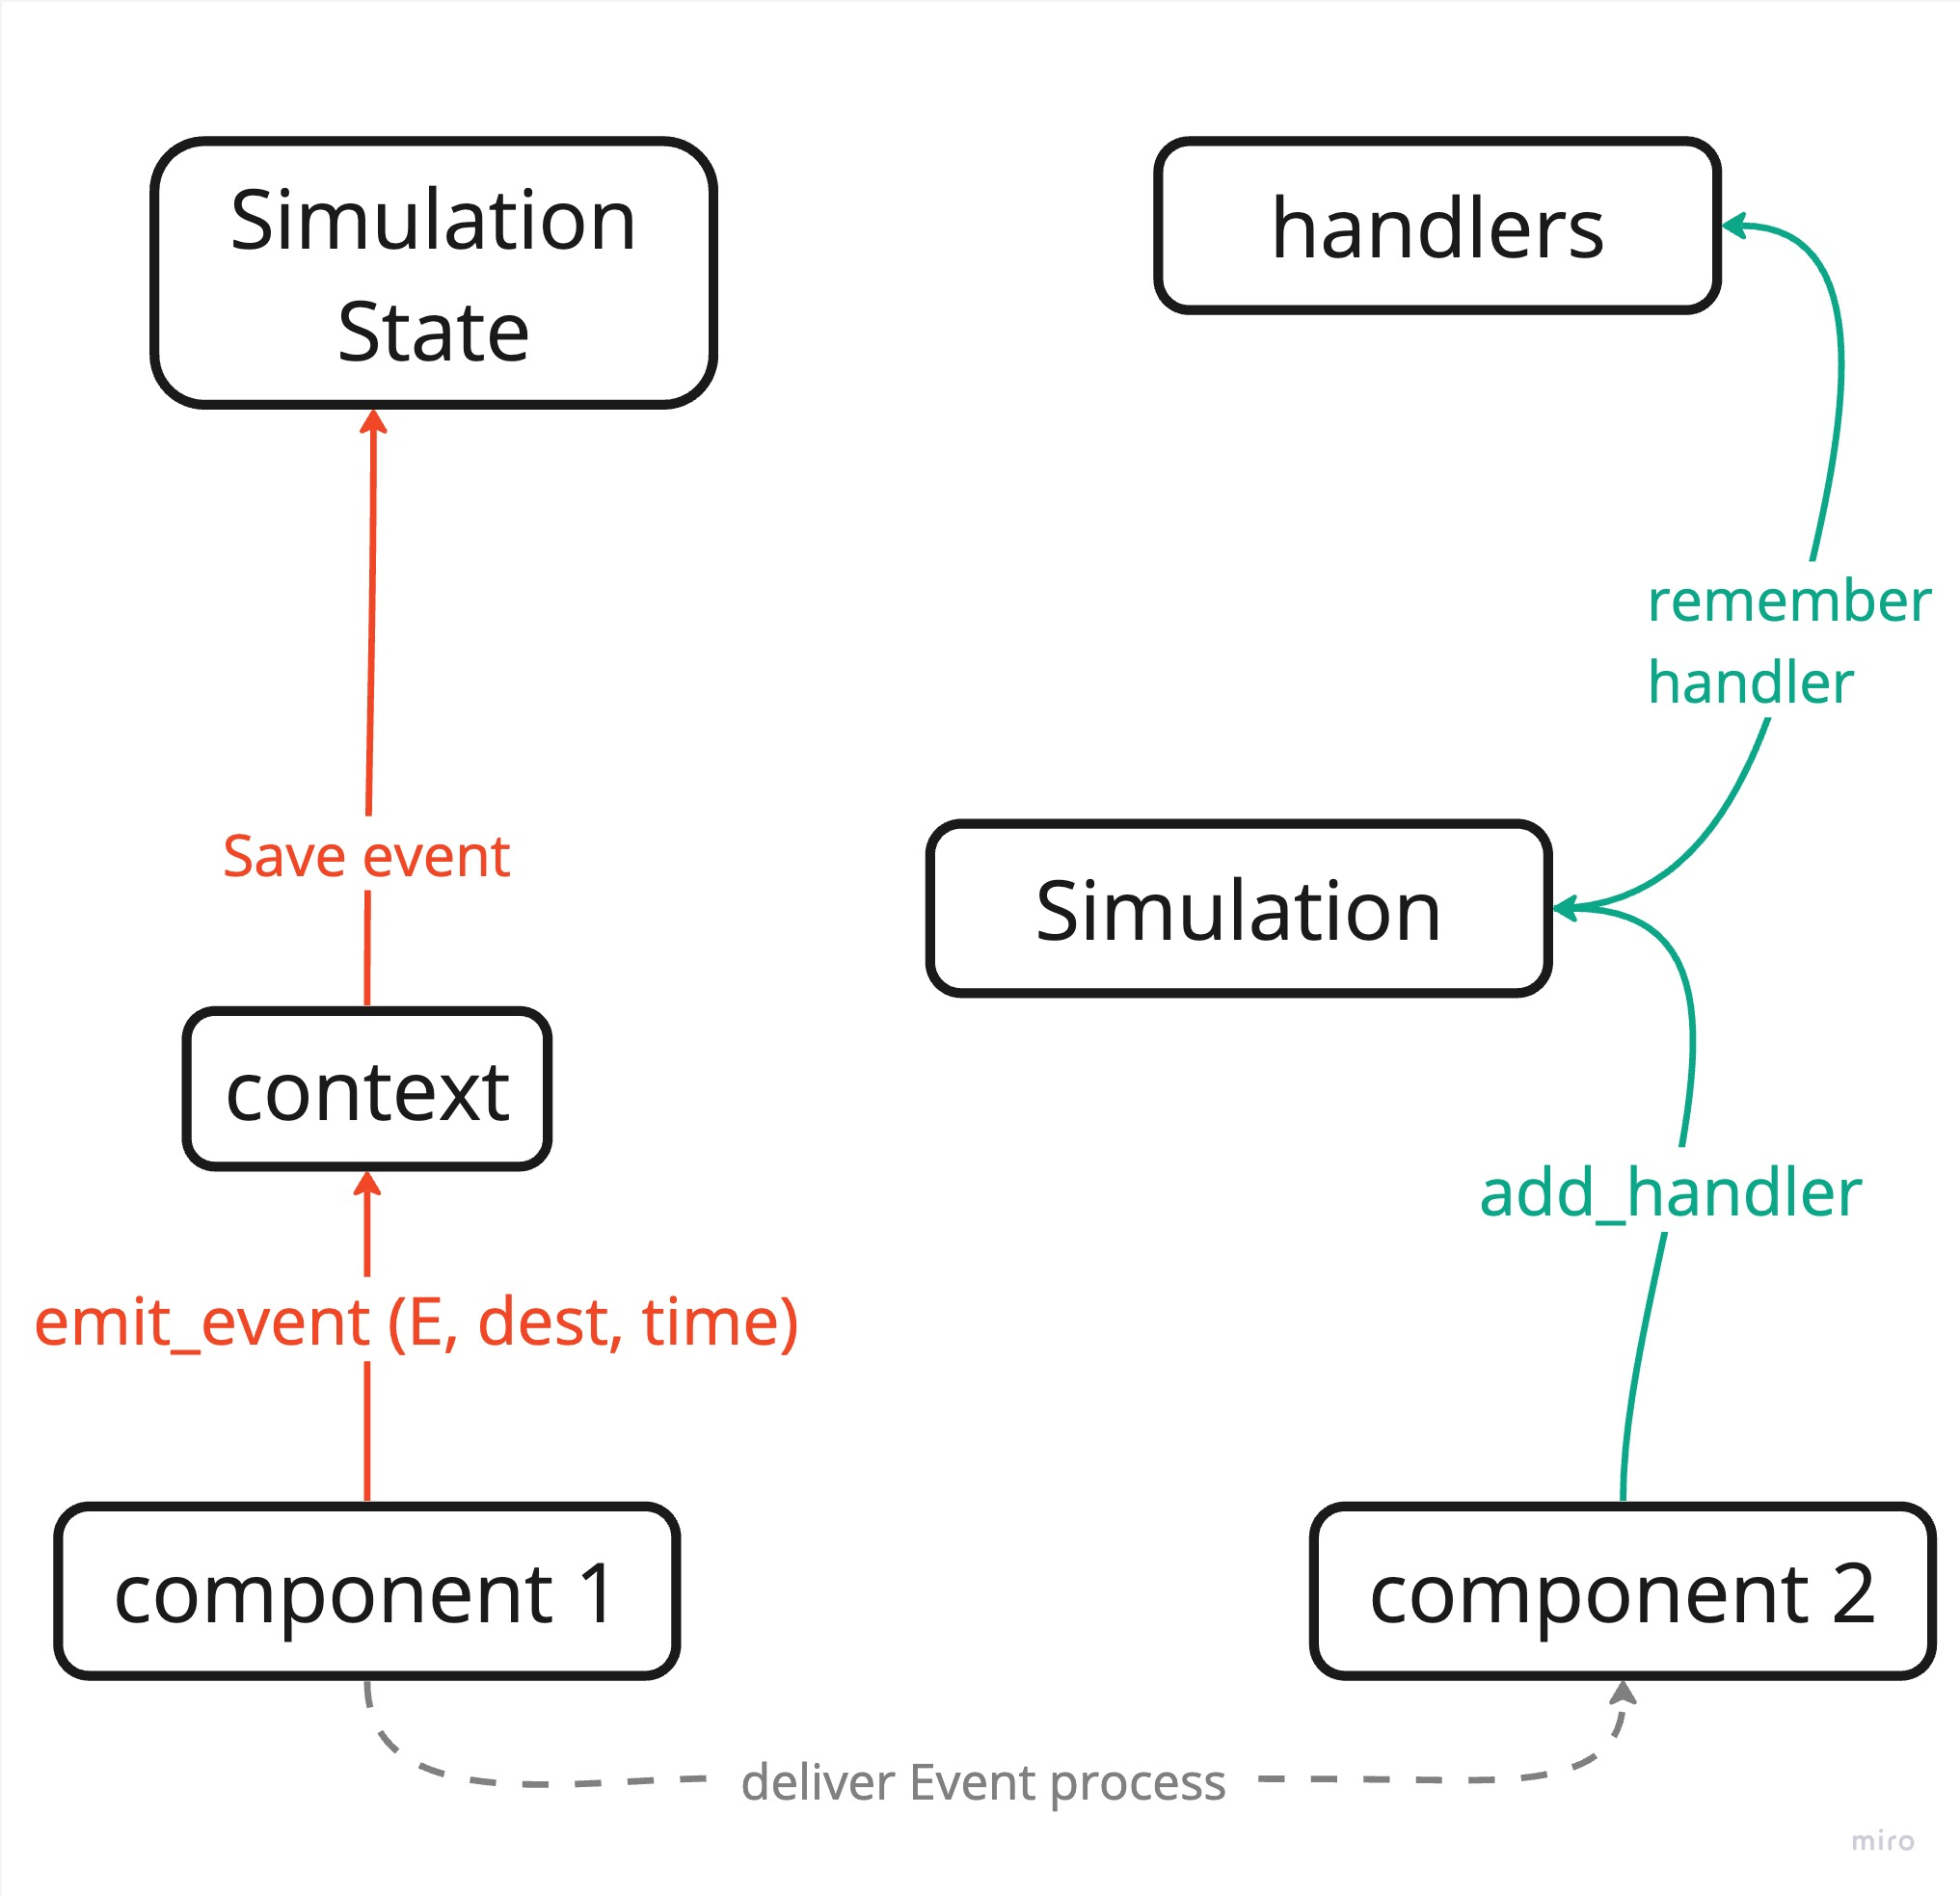
\includegraphics[width=0.72\linewidth]{images/callback_process_3}}{}
		\alt<4>{\hspace{-10.5pt}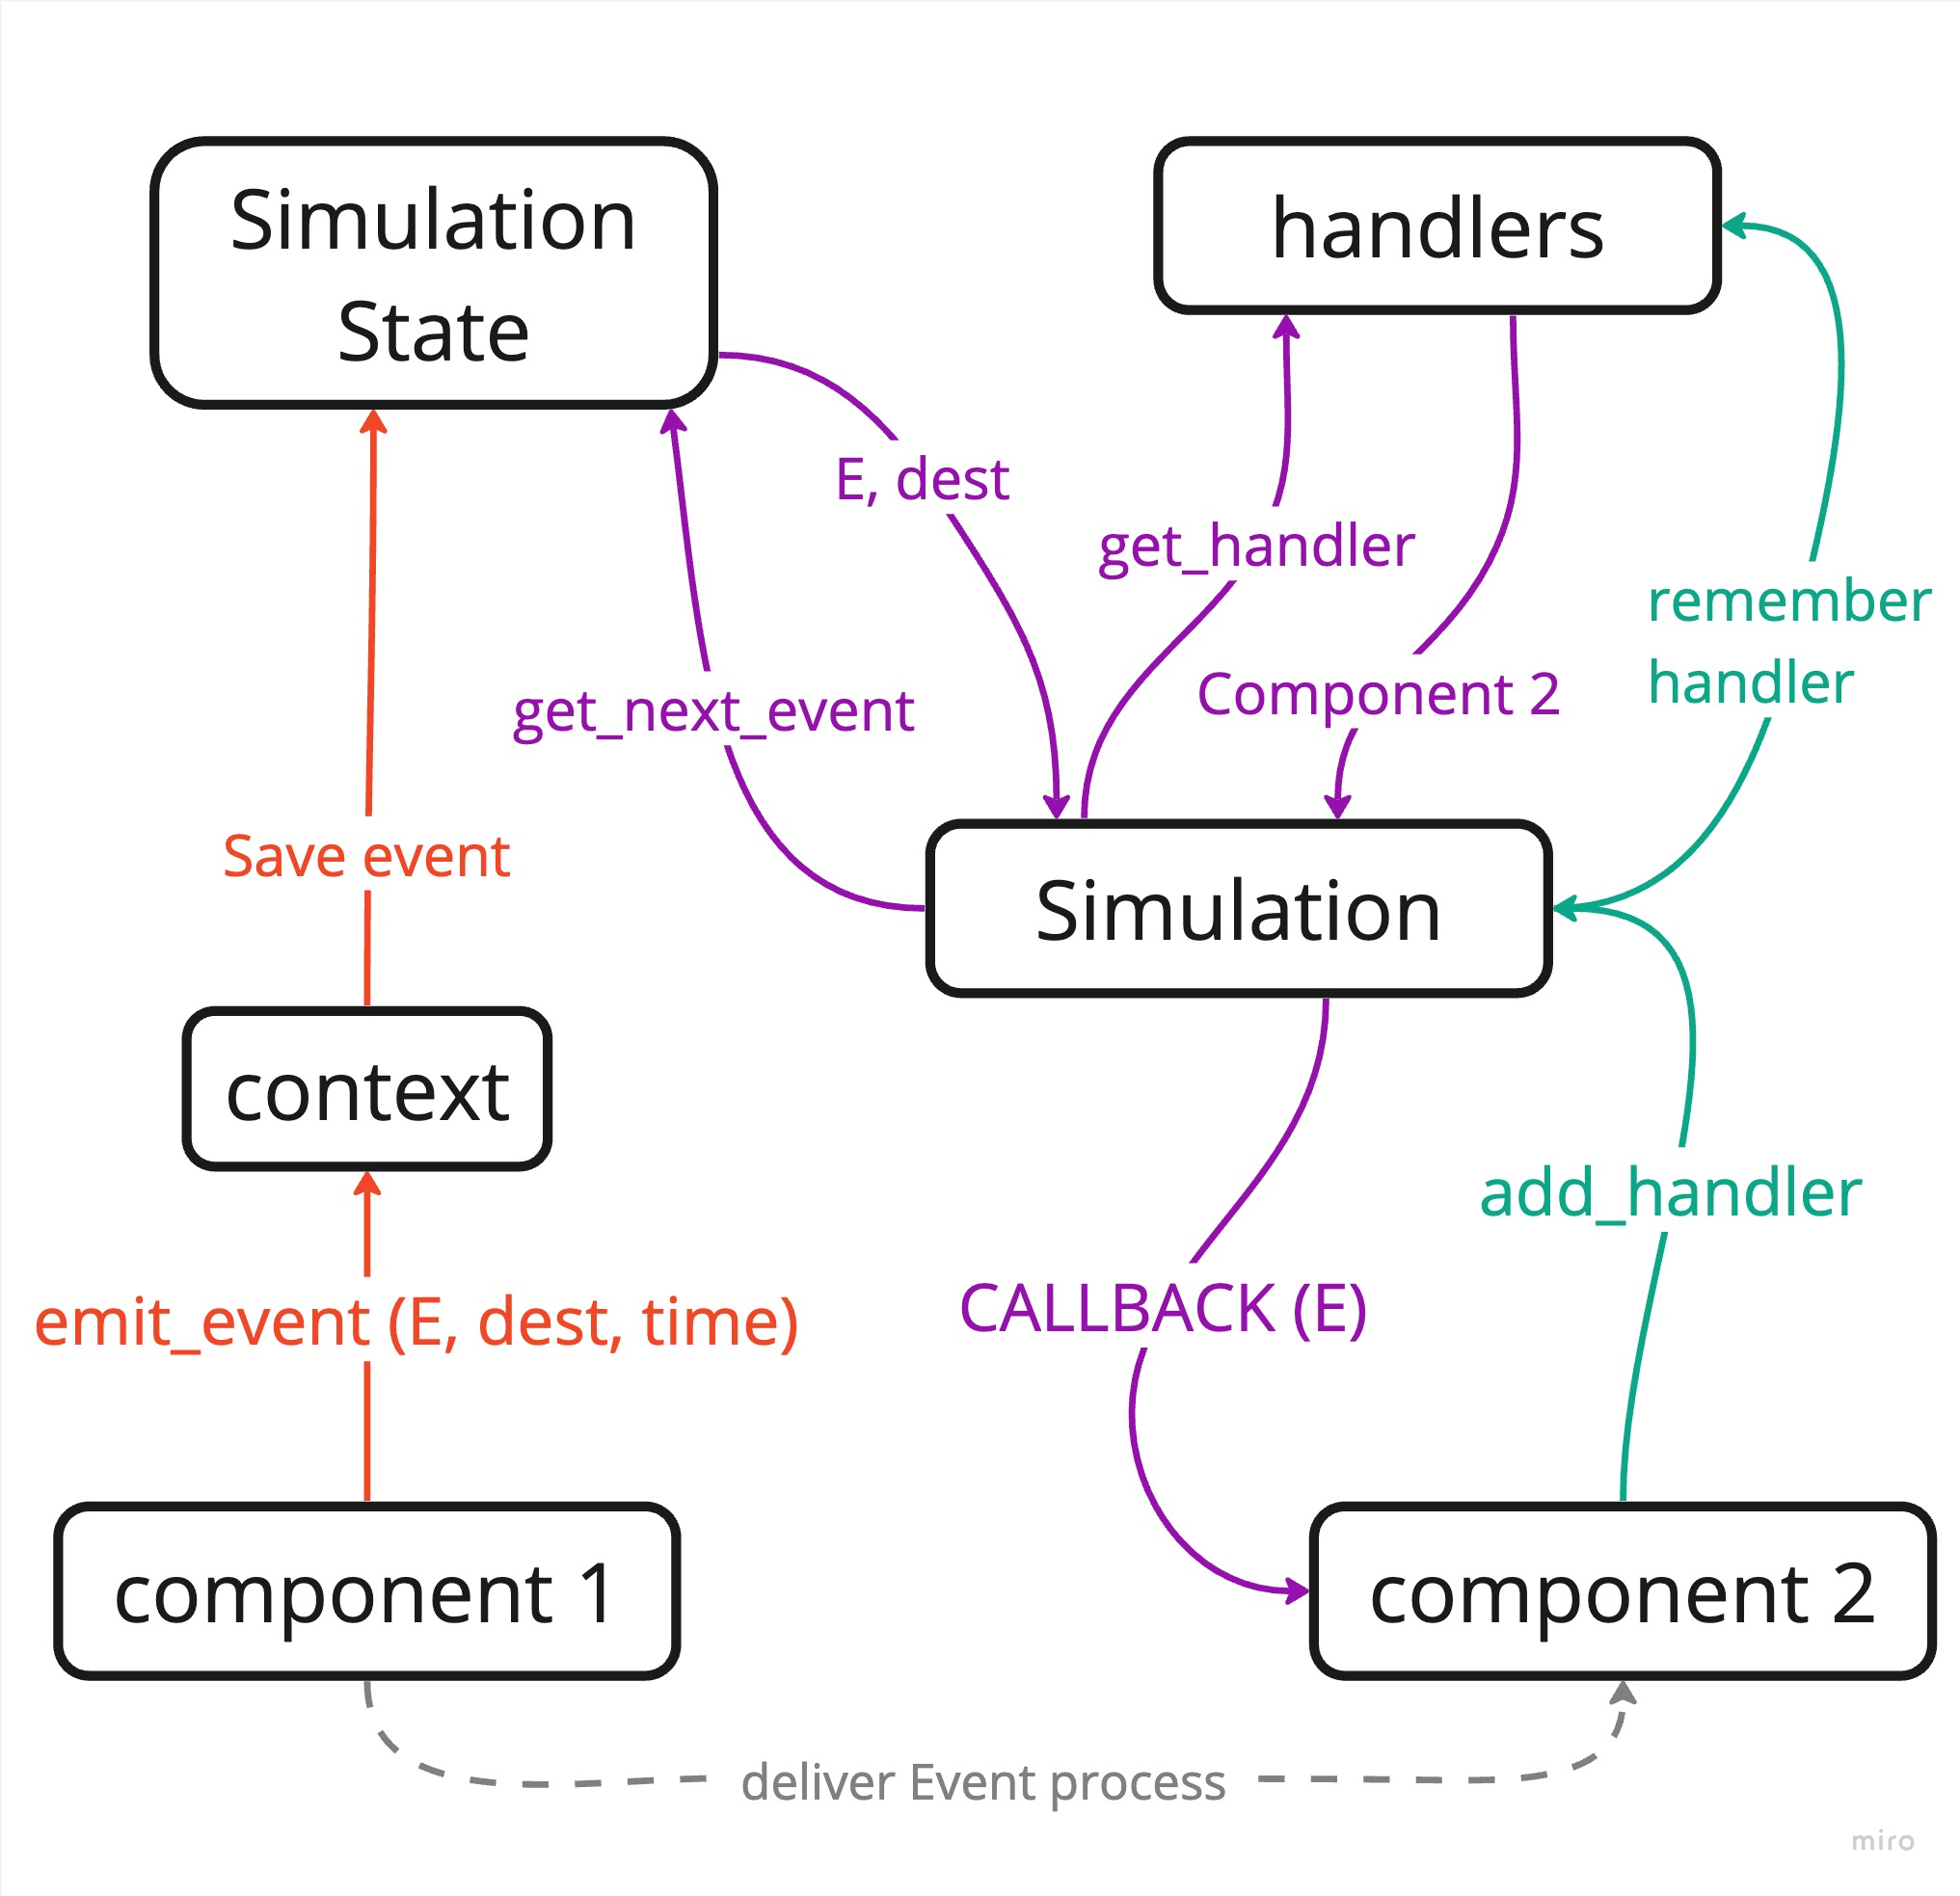
\includegraphics[width=0.72\linewidth]{images/callback_process_4}}{}
	\end{figure}
 \end{frame}



 \section{Внутреннее устройство и реализация}
 \subsection{Асинхронная модель}
 \begin{frame}[fragile]
	\frametitle{\insertsection} 
	\framesubtitle{\insertsubsection}
	\vspace{-10pt}
	\begin{figure}[H]
		\centering
		\alt<1>{\includegraphics<1>[width=0.9\linewidth]{images/async_process_1}}{}
		\alt<2>{\hspace{-3.5pt}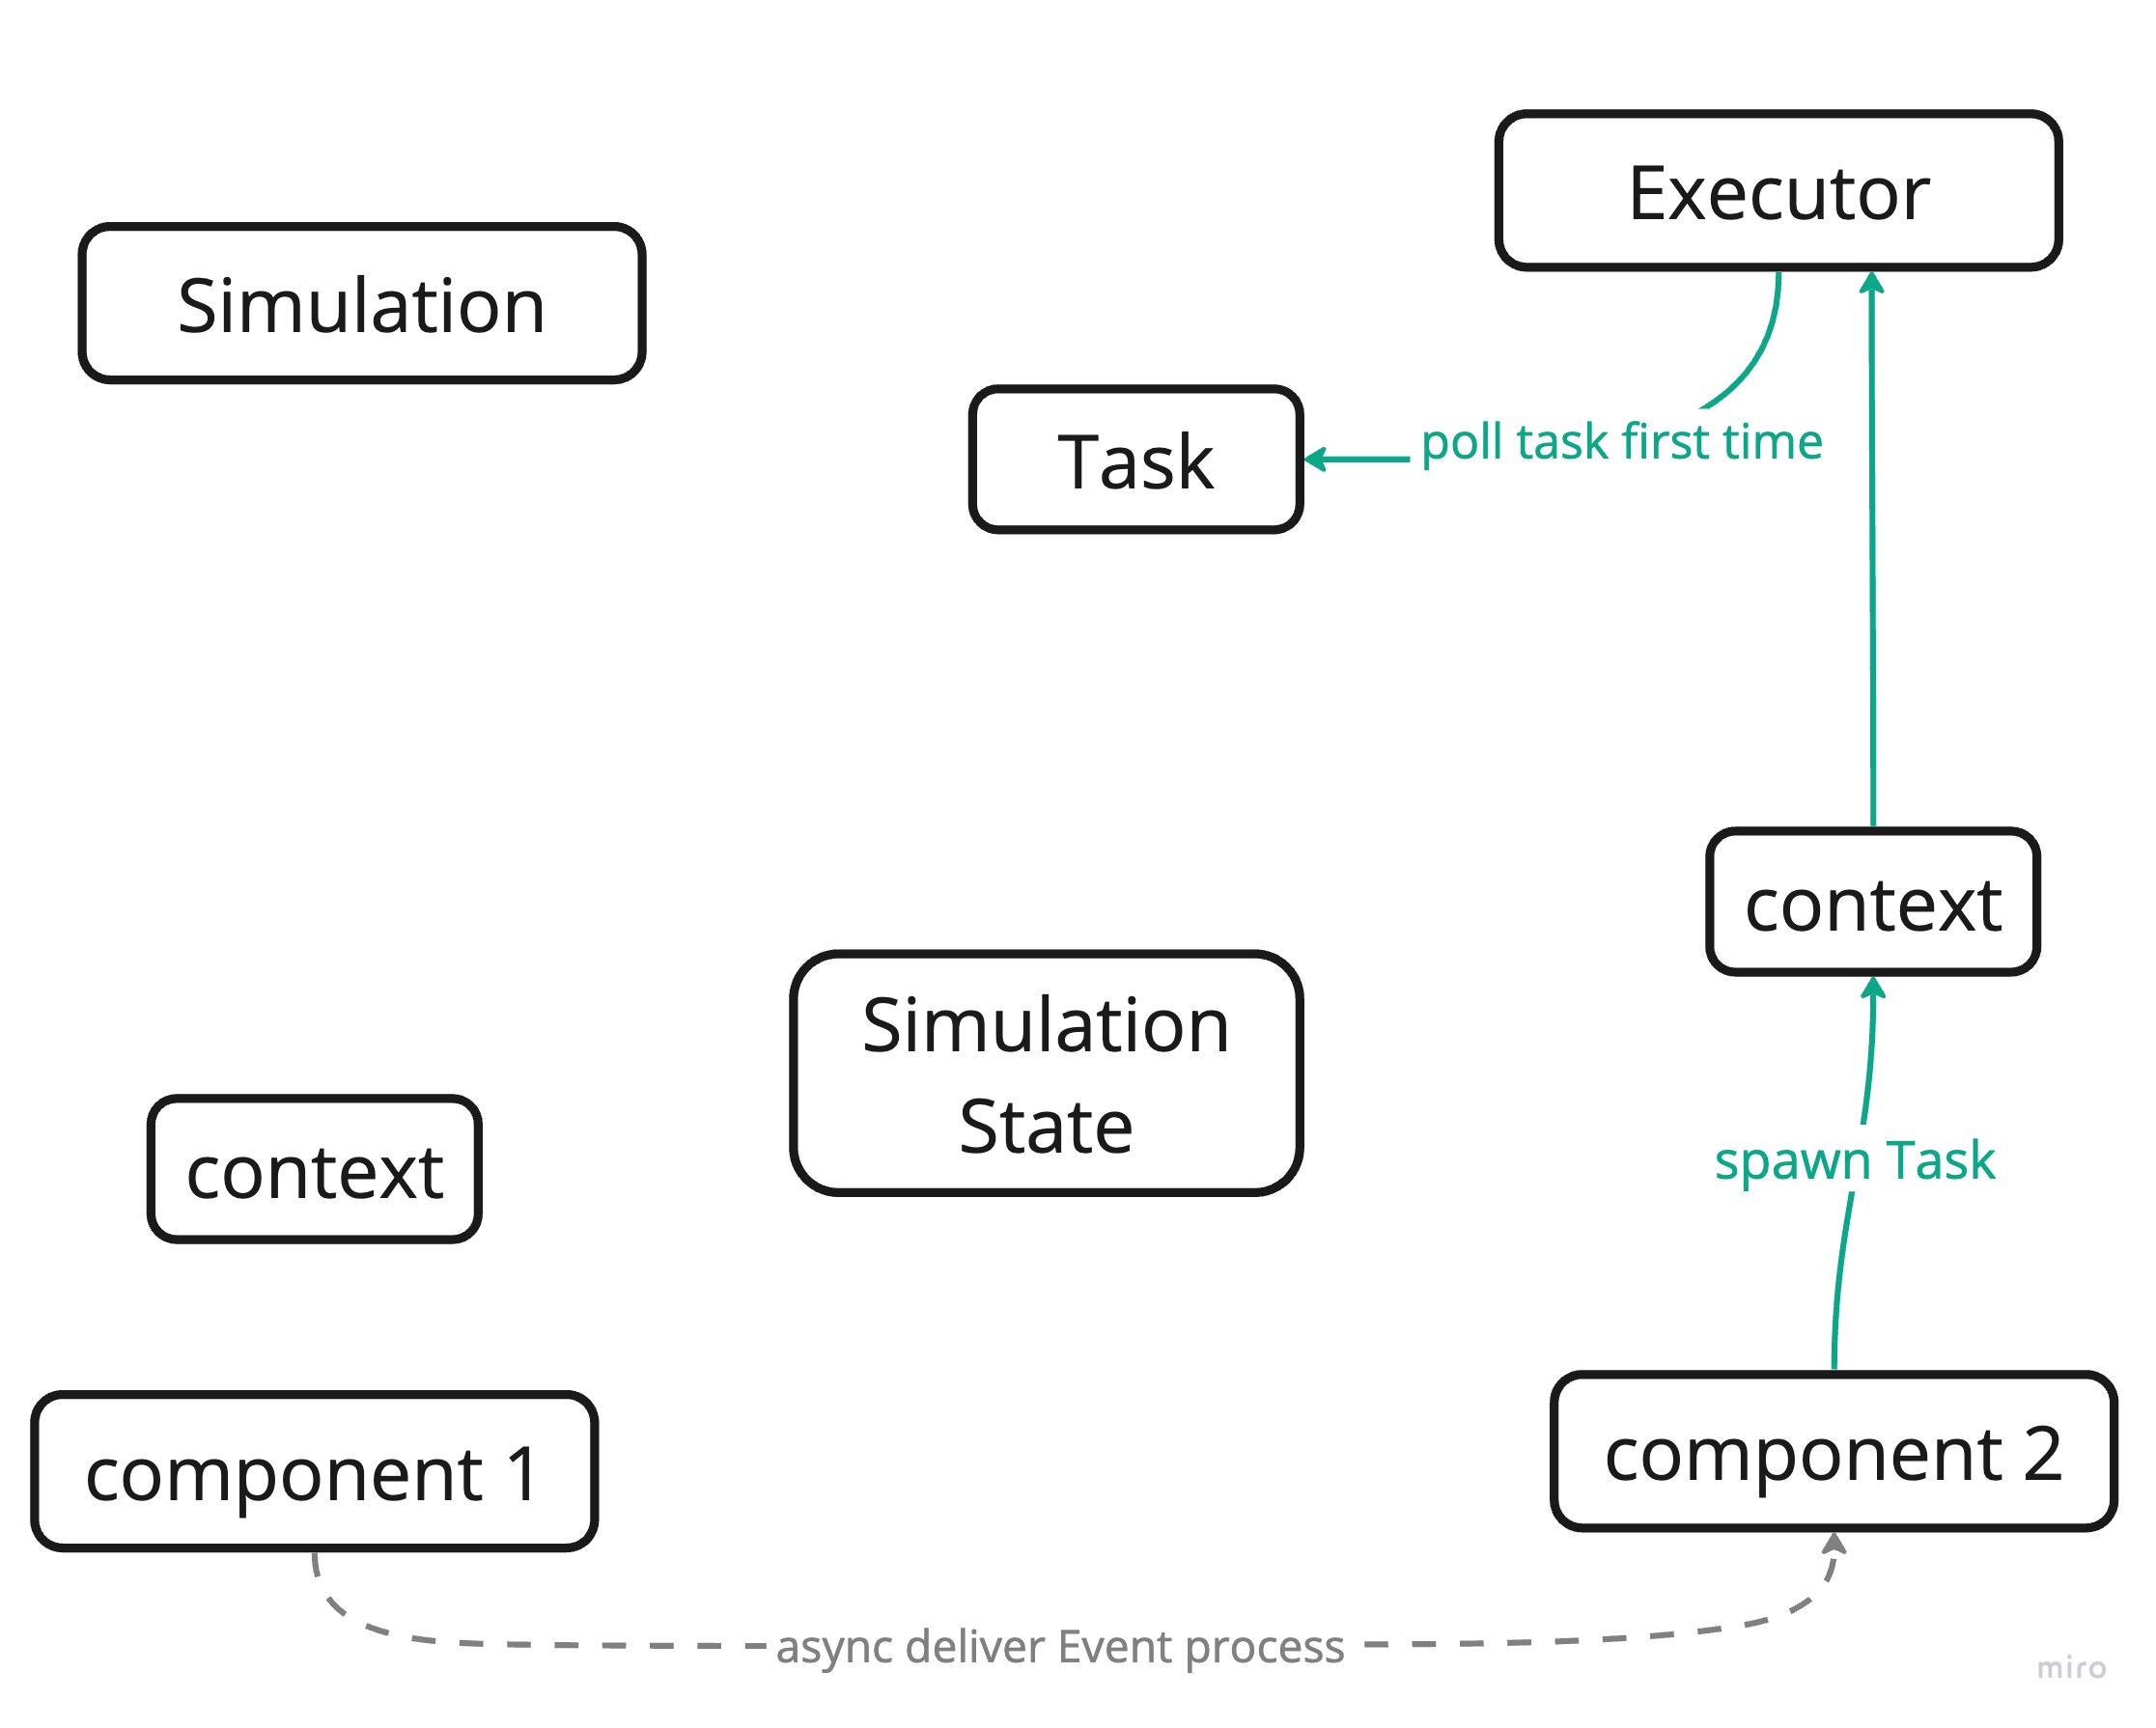
\includegraphics[width=0.9\linewidth]{images/async_process_2}}{}
		\alt<3>{\hspace{-7pt}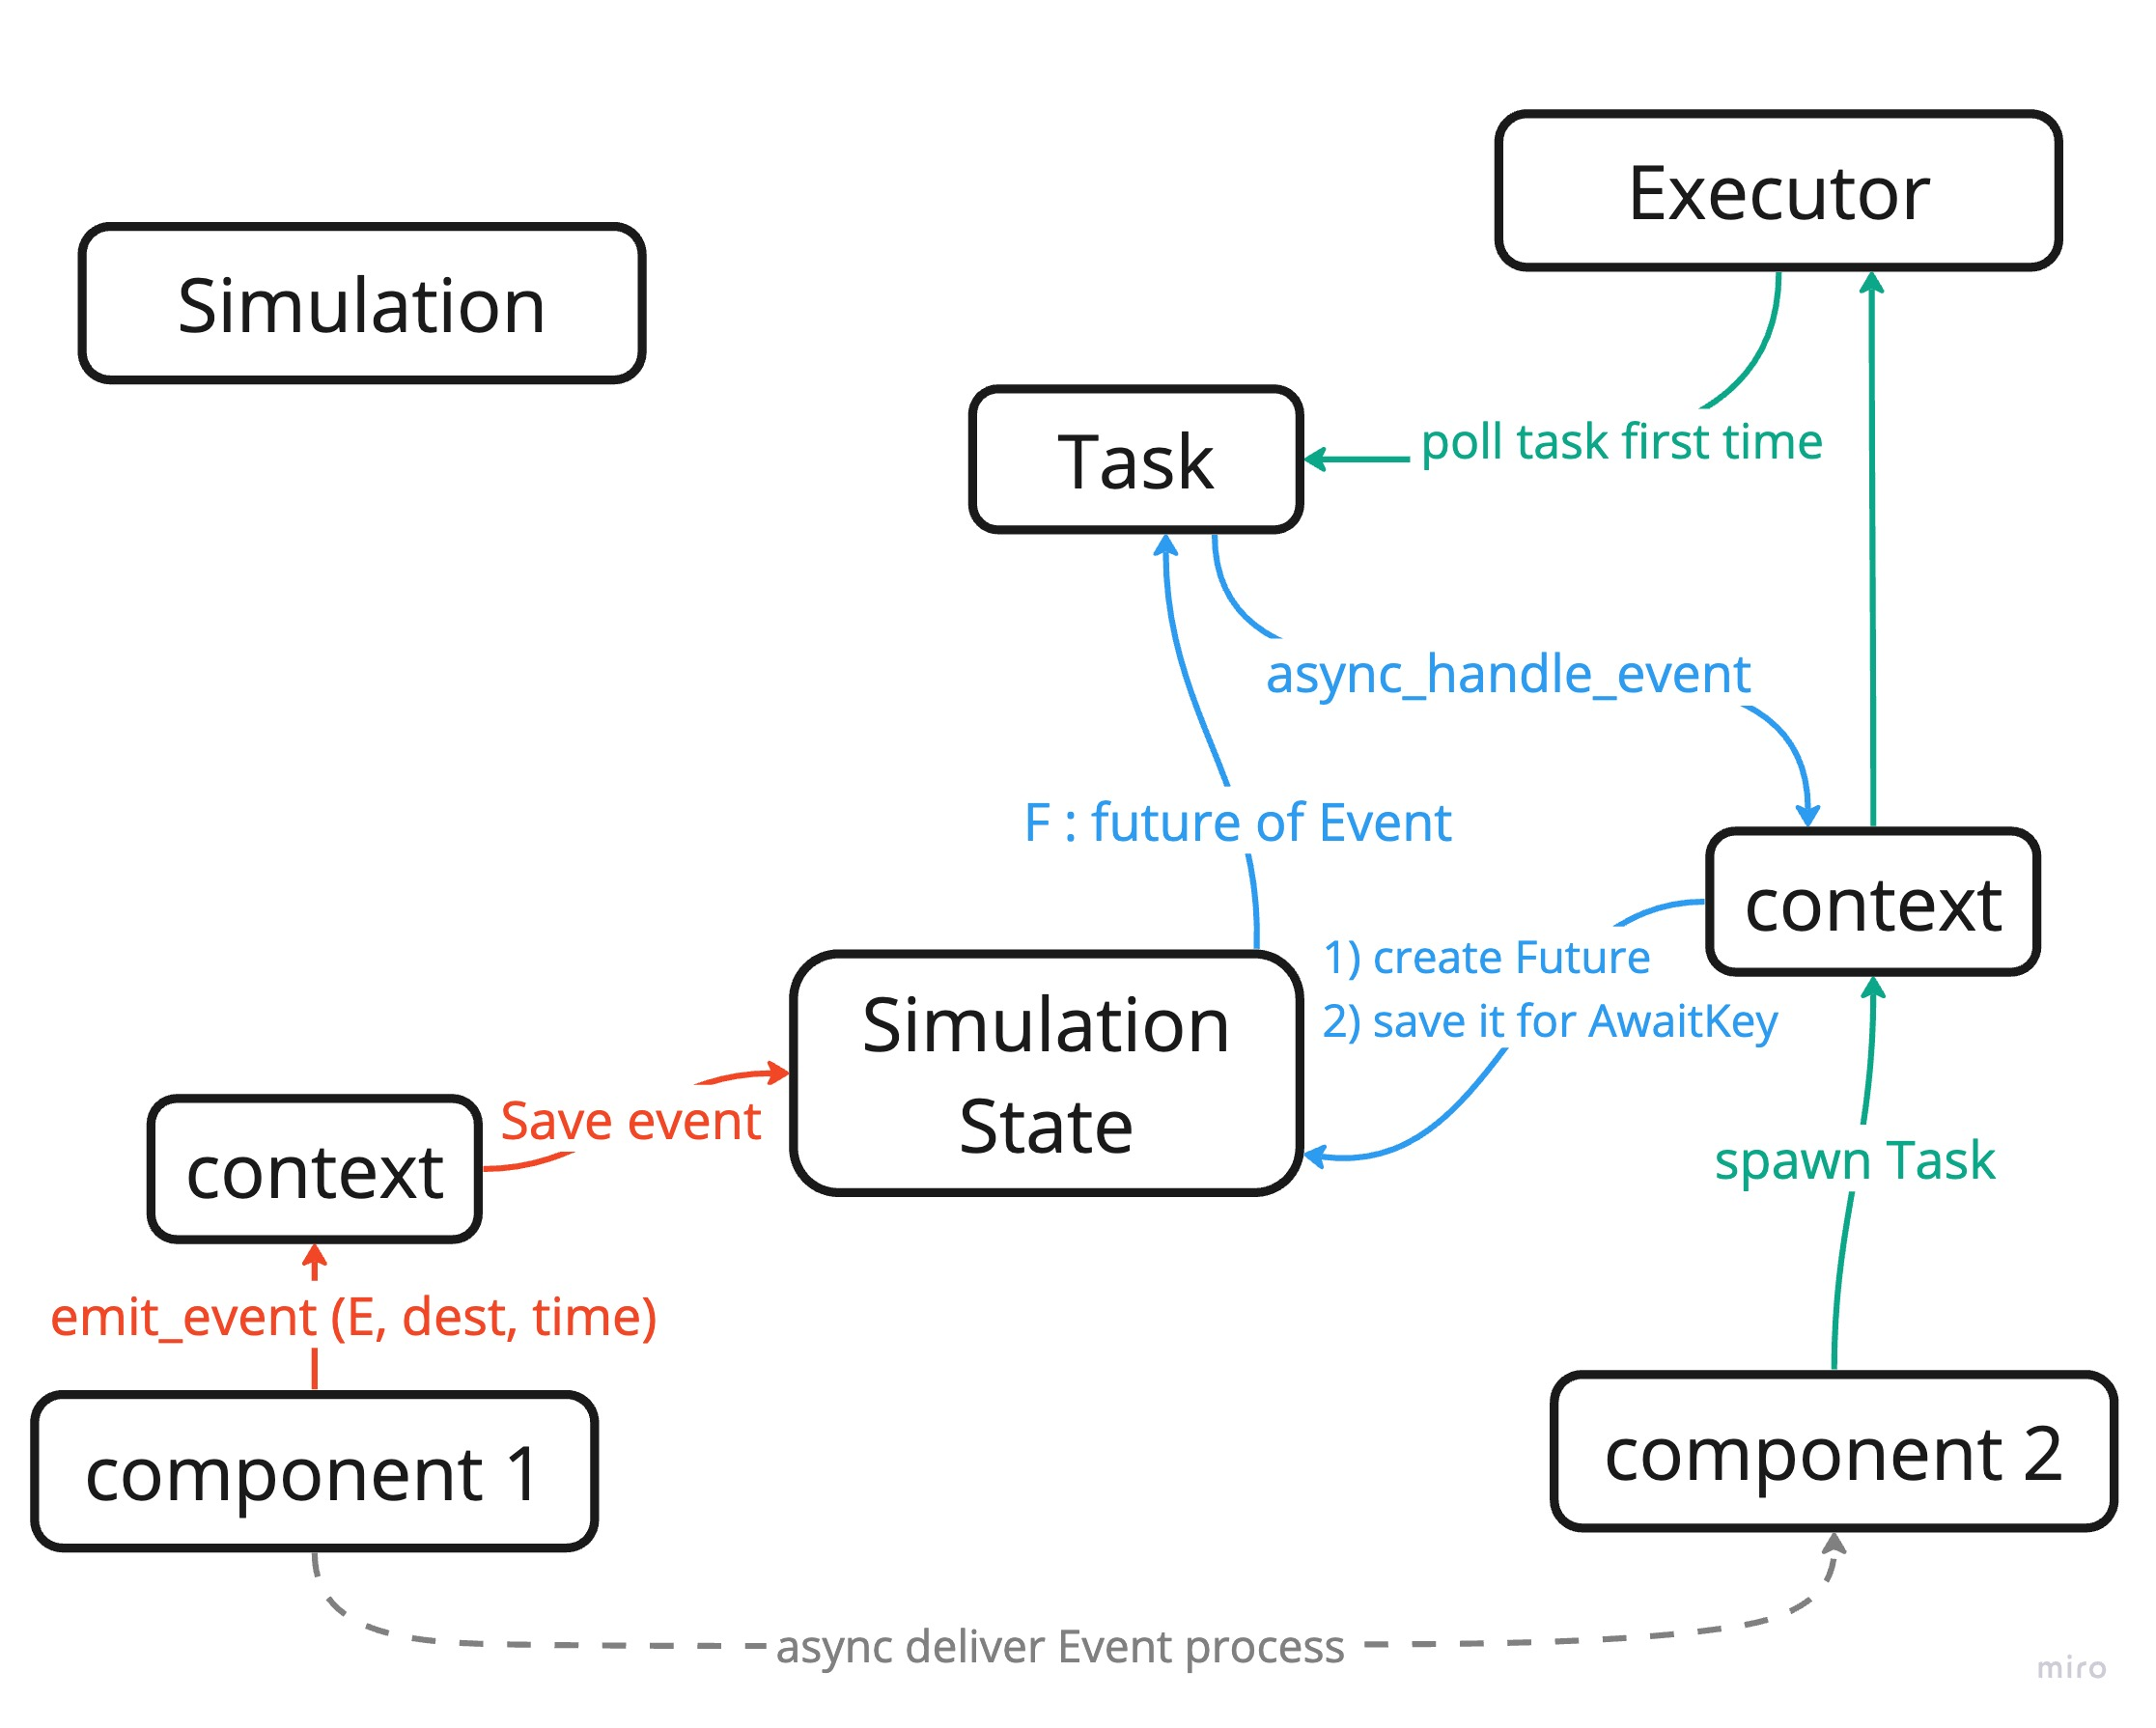
\includegraphics[width=0.9\linewidth]{images/async_process_3}}{}
		\alt<4>{\hspace{-10.5pt}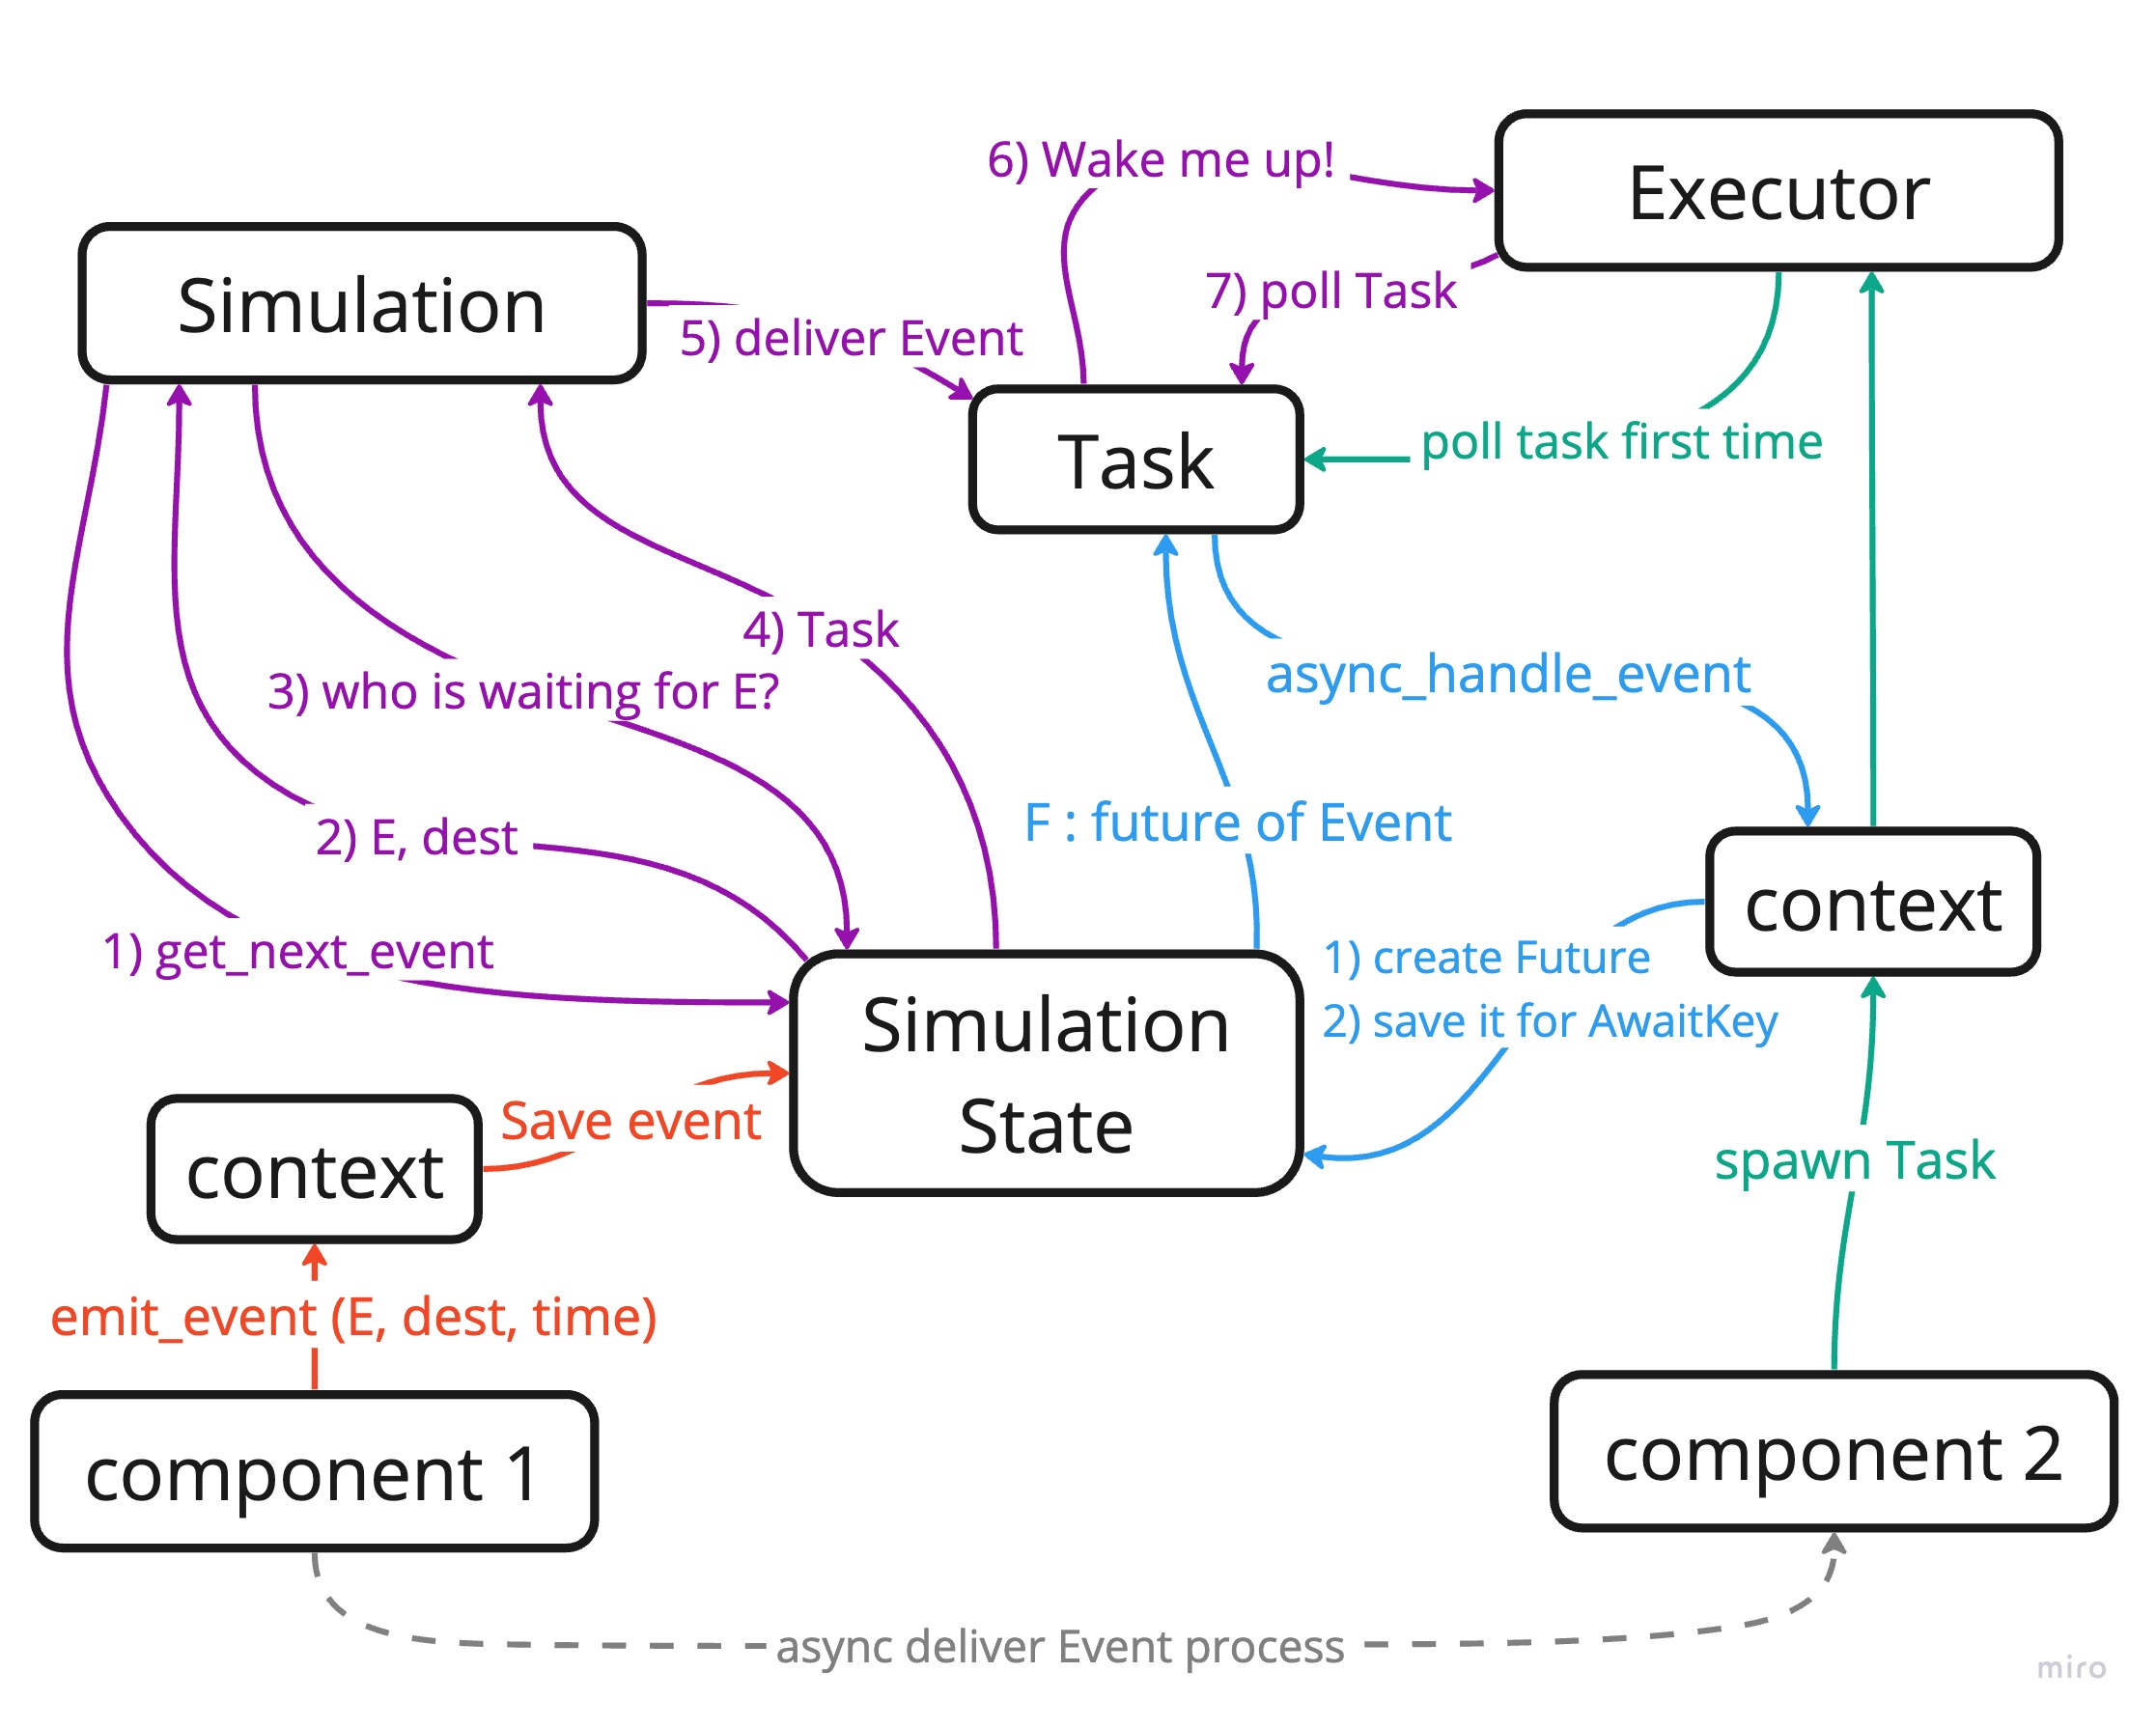
\includegraphics[width=0.9\linewidth]{images/async_process_4}}{}
	\end{figure}
 \end{frame}

 \section{Тестирование}
 \subsection{\texttt{Ping-pong}. Производительность}

 \begin{frame}[fragile]
	\frametitle{\insertsection} 
	\framesubtitle{\insertsubsection}

	\begin{columns}
		\begin{column}[t]{0.3\linewidth}
			\small
			\begin{table}[H]
				\centering
				\begin{tabular}{|c|c|}
					\hline
					Hosts & 100000 \\
					\hline
					Peers per host &  100\\
					\hline
					Iterations & 100 \\ 
					\hline
				\end{tabular}
			\caption*{\hspace{1cm}Аргументы}
			\end{table}
		\end{column}
		\begin{column}[t]{0.6\linewidth}
			\begin{figure}[H]
				\centering
				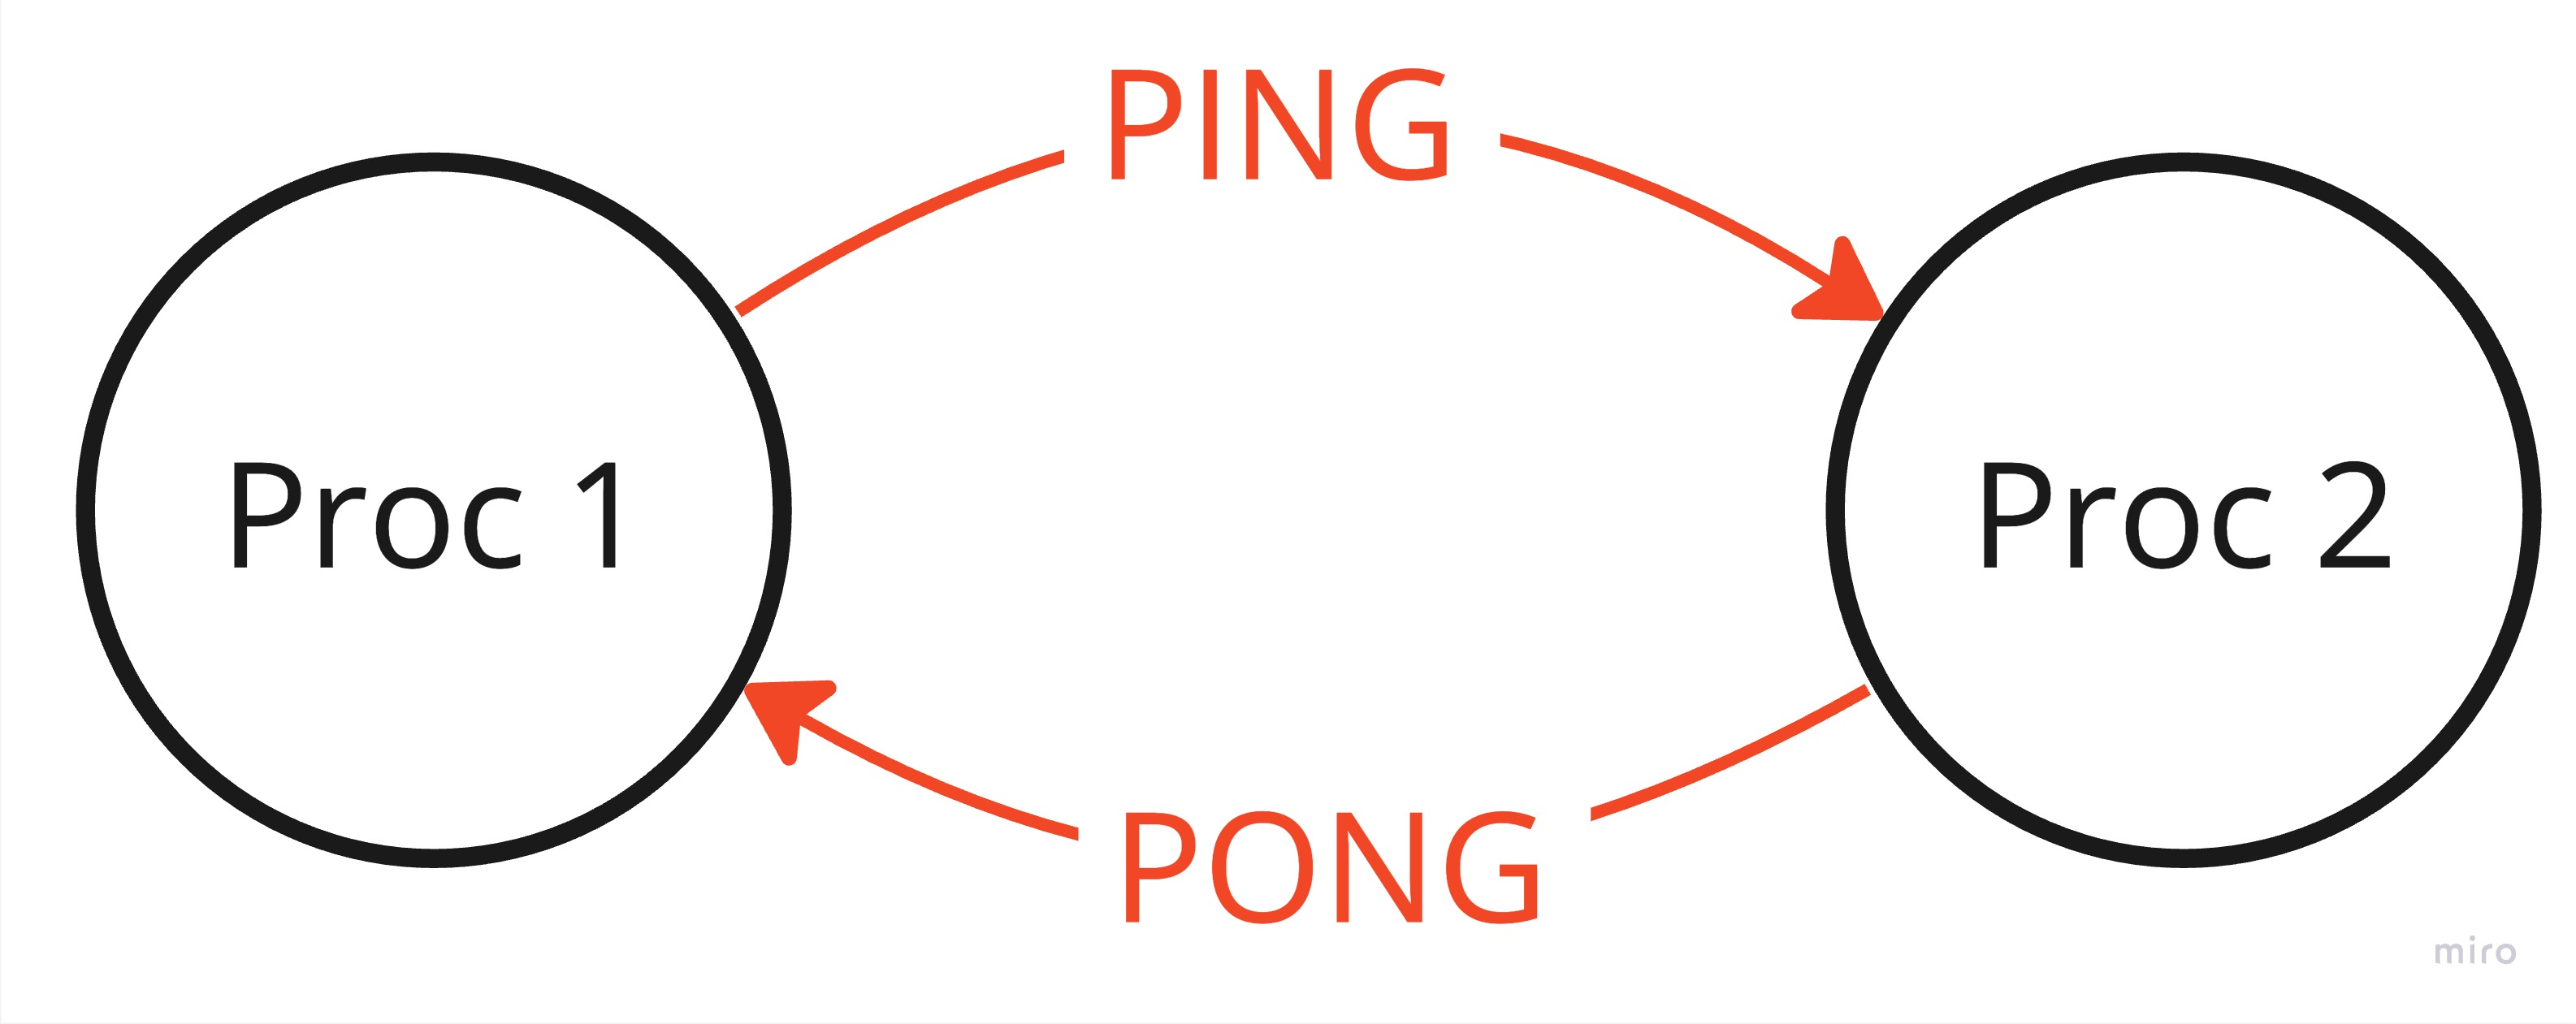
\includegraphics[width=0.8\linewidth]{images/ping_pong_scheme}
			\end{figure}
		\end{column}
	\end{columns}
	
	\begin{table}[H]
		\centering
		\begin{tabular}{|c|c|c|c|}
			\hline
			Example & Elapsed time & Events/s & Iterations/s \\
			\hline
			\texttt{async-ping-pong} & 16.45s & 1234103 & 6.08\\
			\hline
			\texttt{ping-pong} &  8.20s & 2452670 & 12.20\\
			\hline
		\end{tabular}
		\caption*{Сравнение производительности}
	\end{table}
 \end{frame}

 \begin{frame}[fragile]
	\frametitle{\insertsection} 
	\framesubtitle{\insertsubsection}
	\vspace{-0.4cm}
	\begin{figure}
		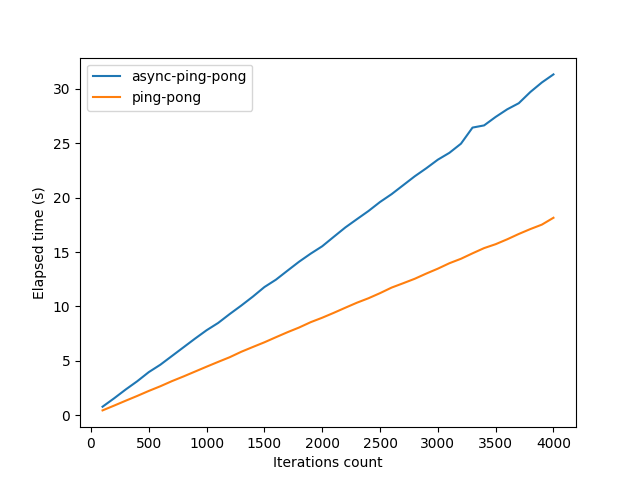
\includegraphics[width=0.8\linewidth]{images/async-ping-pong}
		\caption*{Сравнение производительности}
	\end{figure}
 \end{frame}



 \subsection{\texttt{Master-workers}. Производительность}

 \begin{frame}[fragile]
	\frametitle{\insertsection} 
	\framesubtitle{\insertsubsection}

	\begin{columns}
		\begin{column}[t]{0.3\linewidth}
			\vspace{0.5cm}
			\begin{table}[H]
				\centering
				\begin{tabular}{|c|c|}
					\hline
					Hosts & 100 \\
					\hline
					Tasks &  100000\\
					\hline
				\end{tabular}
			\caption*{Аргументы}
			\end{table}
		\end{column}
		\begin{column}[t]{0.6\linewidth}
			\vspace{-1cm}

			\begin{figure}[H]
				\centering
				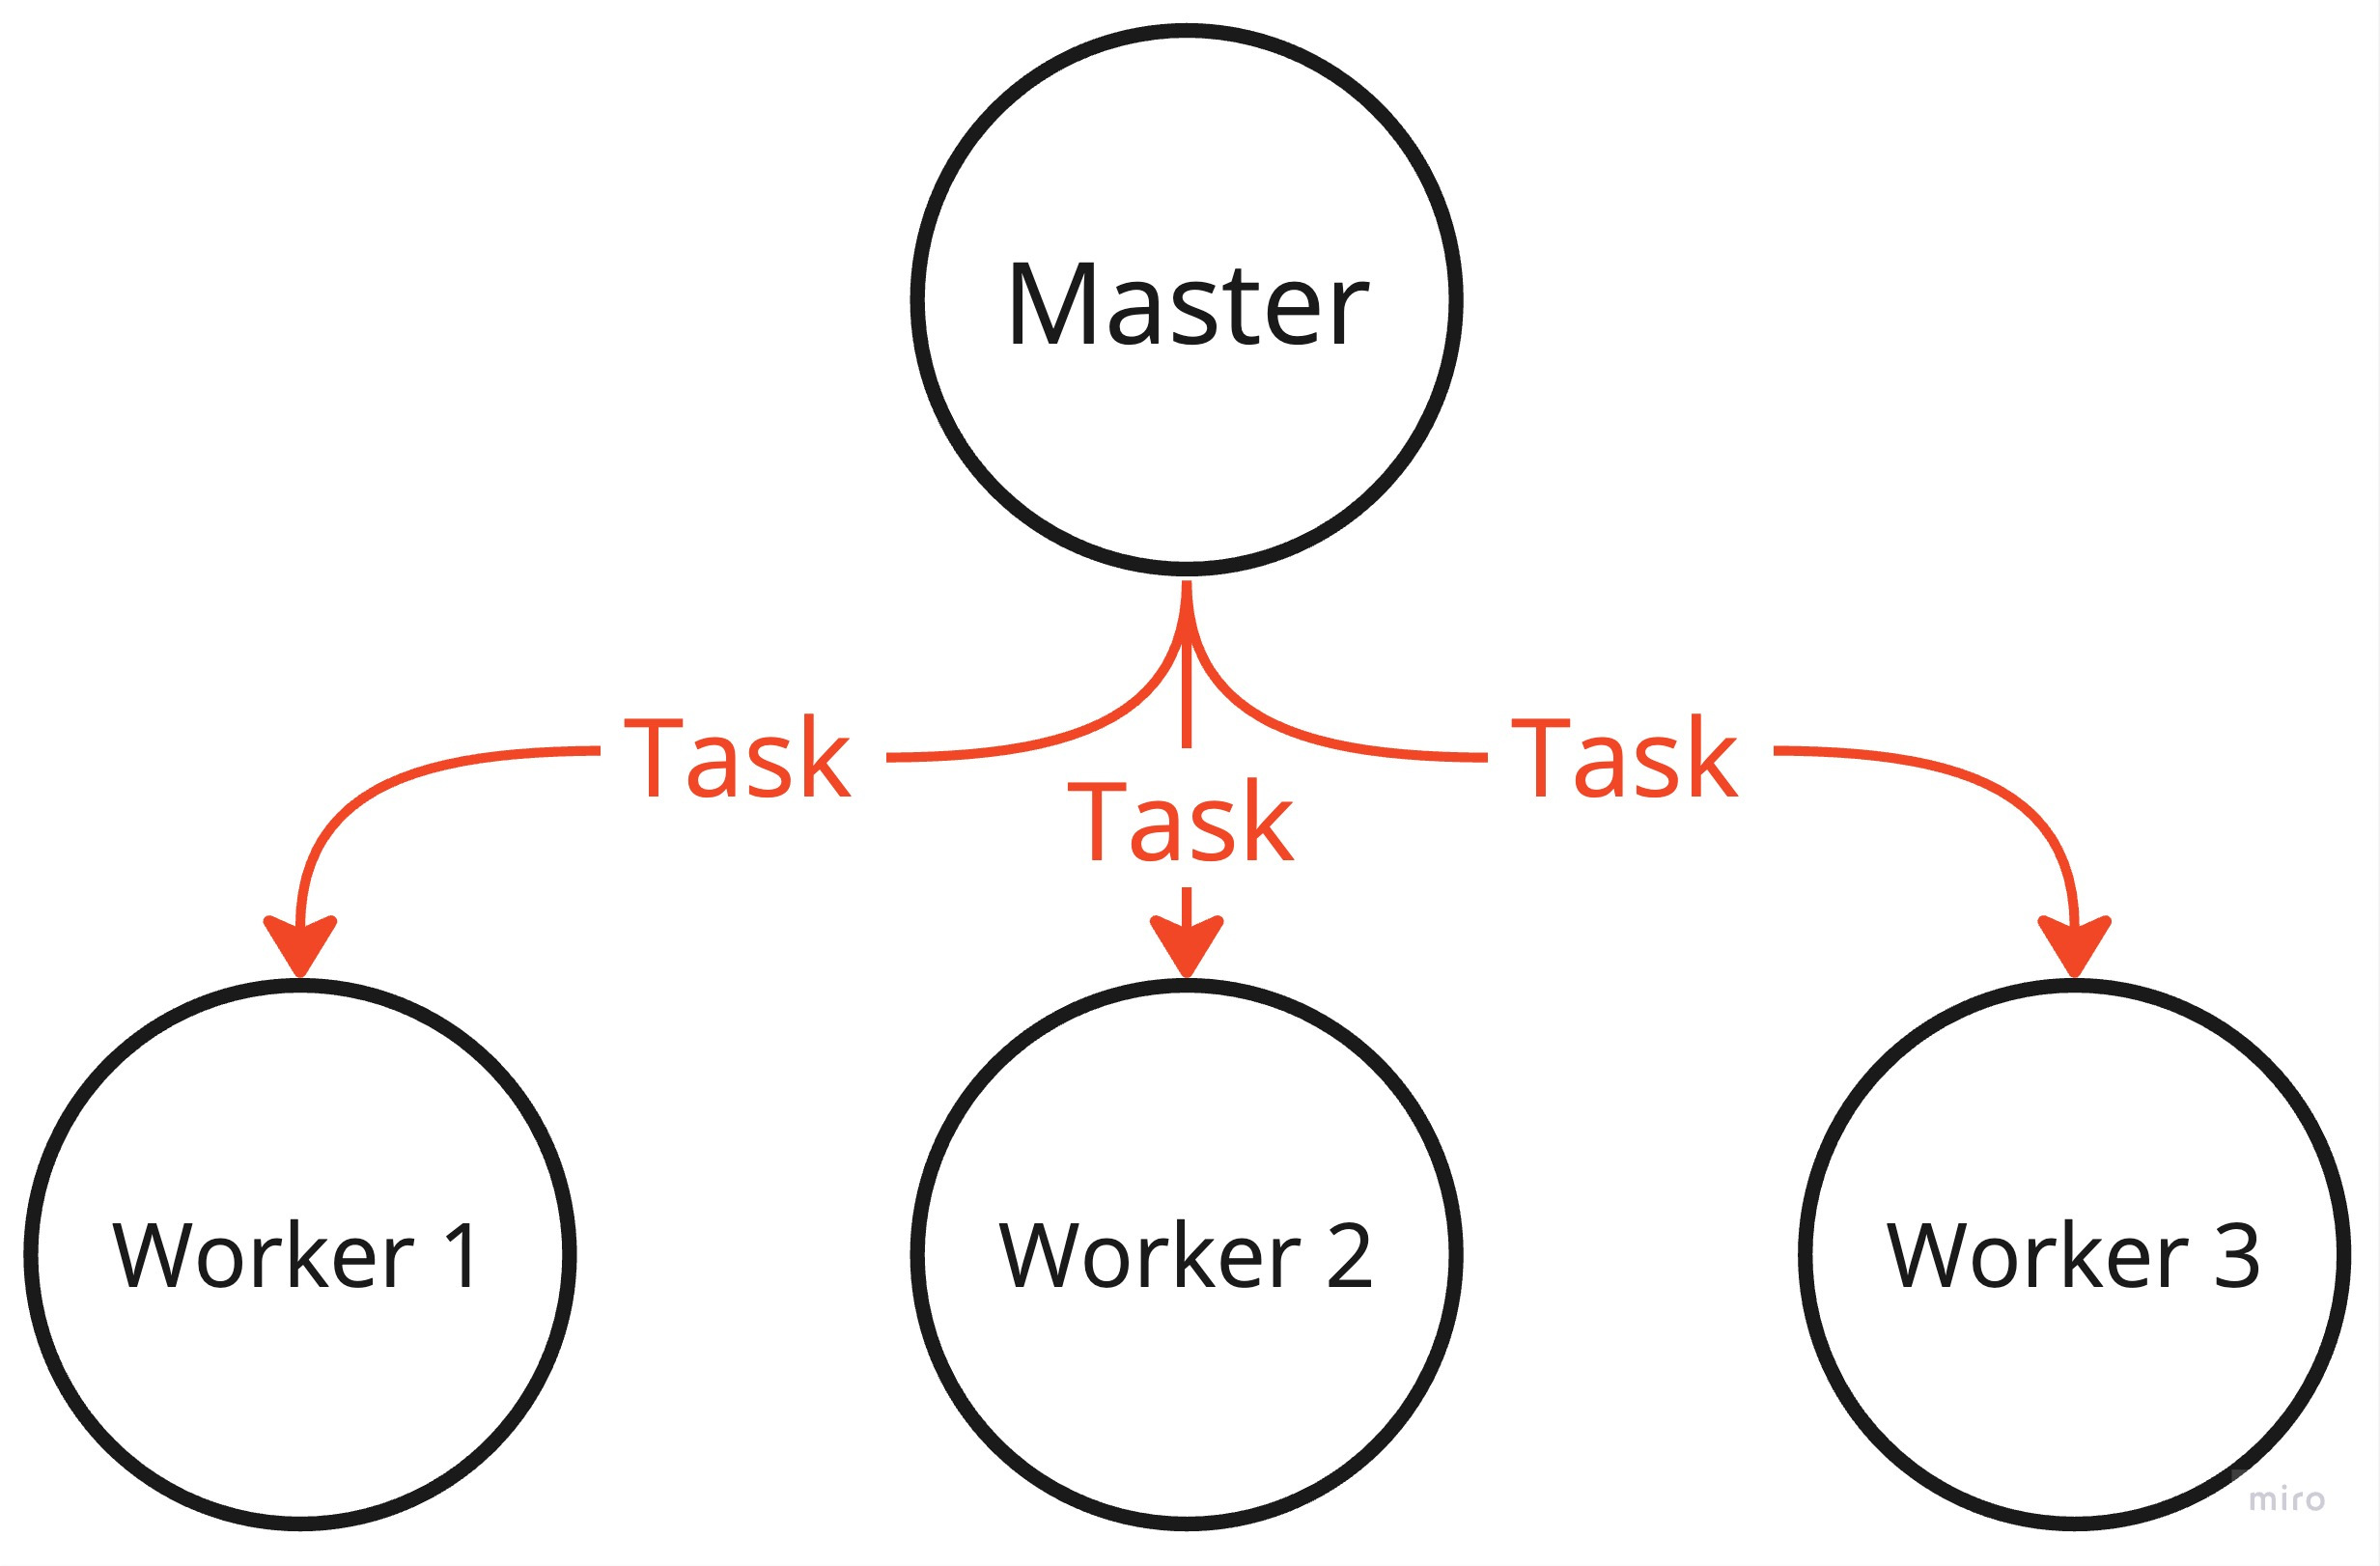
\includegraphics[width=\linewidth]{images/master_workers_scheme}
			\end{figure}
		\end{column}
	\end{columns}
	\vspace{0.3cm}
	\begin{table}[H]
		\small
		\centering
		\begin{tabular}{|c|c|c|c|}
			\hline
			Example & Elapsed time & Scheduling time & Events/s \\
			\hline
			\texttt{async-master-workers} & 5.97s & 4.31s & 285059 \\
			\hline
			\texttt{master-workers}  & 5.19s & 4.31s & 328392 \\
			\hline
		\end{tabular}
		\caption*{Сравнение производительности}
		\label{cmp:master-workers}
	\end{table}
\end{frame}

\subsection{\texttt{Master-workers}. Сравнение кода компонента \texttt{Worker}}

\begin{frame}[fragile]
	\frametitle{\insertsection} 
	\framesubtitle{\insertsubsection}
	\begin{columns}
		\begin{column}[t]{0.55\linewidth}
			\vspace{-0.7cm}
			\begin{figure}
				\centering
				\scriptsize
				\begin{rustcode}[escapeinside={(*@}{@*)}]
pub struct Worker {
 tasks: HashMap<u64, TaskInfo>,
 computations: HashMap<u64, u64>,
 reads: HashMap<u64, u64>,
 writes: HashMap<u64, u64>,
 downloads: HashMap<usize, u64>,
 uploads: HashMap<usize, u64>,
}

fn on_task_request(request);
fn on_data_read_completed(r_id);
fn on_comp_started(comp_id);
fn on_comp_finished(comp_id);
fn on_data_write_completed(r_id);

fn on_data_transfer_completed((*@\textcolor{HSEgreen}{*}@*));
			\end{rustcode}
			\vspace{0cm}
				\caption*{\texttt{master-workers}}
			\end{figure}
		\end{column}
		\vline
		\hspace{2pt}
		\begin{column}[t]{0.57\linewidth}
			\vspace{-0.6cm}
			\begin{figure}
				\centering
				\scriptsize
				\begin{rustcode}
fn on_task_request(req) {
  self.ctx.spawn(
    self.process_task(req));
}

async fn process_task(&self, req: TaskRequest) {
  let mut task = TaskInfo {req};

  self.download_data(&task).await;
  self.read_data(&task).await;
  self.run_task(&task).await;
  self.write_data(&task).await;
  self.upload_result(&task).await;
}
			\end{rustcode}
			\vspace{0.25cm}
				\caption*{\texttt{async-master-workers}}
			\end{figure}
		\end{column}
	\end{columns}
	
\end{frame}

\section{Заключение}

\begin{frame}[fragile]
	\frametitle{\insertsection} 
	\framesubtitle{\insertsubsection}

	\vspace{-0.7cm}
	\begin{columns}
		\begin{column}{1.1\linewidth}
			\begin{itemize}
				\item[\ding{51}] Реализовать эффективное асинхронное расширение для существующего ядра \texttt{dslab-core}.
				\item[\ding{51}] Добавить примеры, написать документацию и тесты.
				\item[\ding{51}] Реализовать примитив синхронизации:  \texttt{<\textless}блокирующая очередь\texttt{>\textgreater} для передачи произвольных данных. 
				\item[\ding{51}] Сделать раздельную сборку ядра $\implies$ классическое ядро не теряет производительность.
				\item[\ding{51}] Сформулировать будущее развитие проекта. 
			\end{itemize}
			\alt<2>{
				\vspace{0.5cm}
				\textbf{Главное достижение:} можно произвольно совмещать оба подхода:
				\begin{itemize}
				\item \texttt{Stateful}-процесс $\implies$ используем асинхронный подход.
				\item \texttt{Stateless}-процесс $\implies$ используем модель \texttt{callback}-ов. 
			\end{itemize}
			}{}
		\end{column}
	\end{columns}
\end{frame}

\section{Приложения}

\begin{frame}{\textbf{Вопросы}}
	
	\begin{enumerate}
		\item \hyperlink{execution}{\nameref{execution}}
		\item \hyperlink{queue}{\nameref{queue}}
		\item \hyperlink{ping-pong}{\nameref{ping-pong}}
		\item \hyperlink{feature}{\nameref{feature}}
		\item \hyperlink{future-plans}{\nameref{future-plans}}
		\item \hyperlink{simgrid}{\nameref{simgrid}}
		\item \hyperlink{dsmodeling}{\nameref{dsmodeling}}
	\end{enumerate}
\end{frame}


\subsection{Execution. \texttt{Stackless}-корутины в \texttt{Rust}. Что такое \texttt{Task}?}\label{execution}
 \begin{frame}[fragile]
	\frametitle{\insertsection} 
	\framesubtitle{\insertsubsection}

	\vspace{-0.7cm}
	\begin{columns}
		\begin{column}[c]{0.40\linewidth}
			\vspace{0.5cm}
			\begin{figure}
				\centering
				\scriptsize
				\begin{rustcode}
fn on_start_action() {
  // do 1
}

fn on_first_event() {
  // do 2
}

fn on_second_event() {
  // do 3
}

/* ... */

on_start_action();
			\end{rustcode}
				\caption*{Синхронный код (разрезан на части разработчиком)}
			\end{figure}
		\end{column}
		\begin{column}[c]{0.05\linewidth}
			\vspace{-1cm}
			$\iff$
		\end{column}
		\begin{column}[c]{0.55\linewidth}
			\vspace{0.3cm}
			\begin{figure}
				\centering
				\scriptsize
				\begin{rustcode}
async fn action() {
  // do 1

  wait_for_first_event().await;

  // do 2 

  wait_for_second_event().await;

  // do 3
}

/* ... */

let future = action();
future.poll(/**/);
			\end{rustcode}
				\caption*{Асинхронный код (разрезан на части компилятором)}
			\end{figure}
		\end{column}
	\end{columns}
 \end{frame}

 \subsection{\texttt{Ping-pong}. Сравнение кода.}\label{ping-pong}

 \begin{frame}[fragile]
	\frametitle{\insertsection} 
	\framesubtitle{\insertsubsection}
	\begin{columns}
		\begin{column}[t]{0.55\linewidth}
			\vspace{-1cm}
			\begin{figure}
				\centering
				\scriptsize
				\begin{rustcode}
pub struct Process {
  iterations: u32,
}

fn on_start(&mut self) {
  let peer = /*random peer*/;
  self.send(Ping {}, peer);
}

fn on_ping(&mut self, from: Id) {
  self.send(Pong {}, from);
}       

fn on_pong(&mut self, from: Id) {
  self.iterations -= 1;
  if self.iterations > 0 {
    let peer = /*choose peer*/
    self.send(Ping {}, peer);
  }
}
			\end{rustcode}
			\vspace{-0.4cm}
				\caption*{\texttt{ping-pong}}
			\end{figure}
		\end{column}
		\begin{column}[t]{0.55\linewidth}
			\vspace{-1cm}
			\begin{figure}
				\centering
				\scriptsize
				\begin{rustcode}
fn on_start(&self) {
  self.ctx.spawn(self.process());
}

fn on_ping(&mut self, from: Id) {
  self.send(Pong {}, from);
}  

async fn process(&self) {
  for _i in 0..self.iterations {
    let peer = /*choose peer*/;
    self.send(Ping {}, peer);

    // stop until receive Pong
    self.ctx.async_handle_event::<Pong>(peer).await;
  }
}
			\end{rustcode}
			\vspace{-0.2cm}
				\caption*{\texttt{async-ping-pong}}
			\end{figure}
		\end{column}
	\end{columns}
 \end{frame}

 \subsection{Примитив синхронизации \texttt{UnboundedBlockingQueue<T>}.}\label{queue}

 \begin{frame}[fragile]
	\frametitle{\insertsection} 
	\framesubtitle{\insertsubsection}

	\vspace{0cm}
	\begin{columns}
		\begin{column}{\linewidth}
			\begin{figure}
				\centering 
				\scriptsize
				\begin{rustcode}
pub struct Worker {
  task_chan: UnboundedBlockingQueue<TaskInfo>,
}

fn on_task_request(&self, task_info: TaskInfo) {
  self.task_chan.send(task_info);
}

async fn work_loop(&self) {
  loop {
    let task_info = self.task_chan.receive().await;
    /* process task */
  }
}
				\end{rustcode}
				\vspace{-0.2cm}
				\caption*{Использование \texttt{UnboundedBlockingQueue<T>} как буфер для задач}
			\end{figure}
		\end{column}
	\end{columns}

 \end{frame}


 \subsection{Раздельная сборка. Feature \texttt{async-core}.}\label{feature}
 \begin{frame}[fragile]
	\frametitle{\insertsection}
	\framesubtitle{\insertsubsection}
	\small

	Пакет \texttt{dslab-core} можно подключить с разными опциями:
	\begin{itemize}
		\item \small \texttt{dslab-core = \{ path = "../dslab-core" \}} -- асинхронность не поддерживается. Максимальная производительность. 
		\item \small \texttt{dslab-core = \{ path = "../dslab-core", features = ["async\_core"] \} } -- поддерживается весь асинхронный интерфейс. Скорость симуляции снижена.
	\end{itemize}
 \end{frame}

 \subsection{Планы на будущее. Дальнейшее развитие проекта.}\label{future-plans}
 \begin{frame}[fragile]
	\frametitle{\insertsection}
	\framesubtitle{\insertsubsection}

\begin{itemize}
	\setlength{\itemsep}{0.8em}
	\item Повышение удобства синтаксиса.
	\item Увеличение производительности симуляции.
    \item Расширение асинхронной функциональности: 
	\begin{itemize}
		\setlength{\itemsep}{0.5em}
		\item[\small\textgreater] \texttt{yield} -- уйти в конец очереди планировщика без продвижения по времени. 
		\item[\small\textgreater] \texttt{Cancellation}. Возможность отменять задачи.  
	\end{itemize}
	\item Расширение  \texttt{<\textless}стандартных\texttt{>\textgreater} асинхронных инструментов:
	\begin{itemize}
		\setlength{\itemsep}{0.5em}
		\item[\small\textgreater] Полноценный канал из \texttt{Go}
		\item[\small\textgreater] \texttt{ConditionVariable?} 
	\end{itemize}
\end{itemize}
 \end{frame}

 \subsection{Сравнение с аналогами. \texttt{SimGrid}.}\label{simgrid}
\begin{frame}[fragile]
	\frametitle{\insertsection} 
	\framesubtitle{\insertsubsection}

	\vspace{-1cm}
	\begin{columns}
		\begin{column}{1.1\linewidth}
			\begin{figure}
				\centering 
				\scriptsize
				\begin{cppcode}
void Process(int id, Mailbox* in, vector<Mailbox*> peers, 
 int iters) {
  // wait for Start message
  auto* msg = in->get<Message>();
  bool stopped = false;
  bool wait_reply = false;
  while (!stopped) {
    if (pings_to_send > 0 && !wait_reply) {
      MailBox* peer_mailbox = /* choose peer */;
      peer_mailbox->put_init(new Message(/*create message*/));
      wait_reply = true;
      pings_to_send -= 1;
    }
    msg = in->get<Message>();
    if (msg->type == MessageType::PING) {/* handle PING */} 
    else if (msg->type == MessageType::PONG) {/* handle PONG */} 
    else if (msg->type == MessageType::STOP) { stopped = true; }
  }
}
				\end{cppcode}
				\vspace{-0.2cm}
				\caption*{Код процесса \texttt{ping-pong} в фреймворке \texttt{SimGrid}}
			\end{figure}
		\end{column}
	\end{columns}
\end{frame}
\subsection{Как устроено дискретно-событийное моделирование}\label{dsmodeling}
\begin{frame}
    \frametitle{\insertsection} 
	\framesubtitle{\insertsubsection}

	\begin{figure}
		\centering
		{
		\includegraphics<1>[width=\linewidth]{images/event_pipeline_0}
		\includegraphics<2>[width=\linewidth]{images/event_pipeline_1}
		\includegraphics<3>[width=\linewidth]{images/event_pipeline_2}
		\includegraphics<4>[width=\linewidth]{images/event_pipeline_3}
		\includegraphics<5>[width=\linewidth]{images/event_pipeline_4}
		\includegraphics<6>[width=\linewidth]{images/event_pipeline_5}
		\includegraphics<7>[width=\linewidth]{images/event_pipeline_6}
		\includegraphics<8>[width=\linewidth]{images/event_pipeline_7}
		\includegraphics<9>[width=\linewidth]{images/event_pipeline_8}
		\includegraphics<10>[width=\linewidth]{images/event_pipeline_9}
		}
		\caption*{Исполнение симуляции}
	\end{figure}
    \end{frame}
\end{document}